%%%%%%%%%%%%%%%%%%%%%%%%%%%%%%%%%%%%%%%%%%%%%%%%%%%%%%%%%%%%%%%%%%%%%%%%%%%%%%%%%%%%%%%%%
%%                                                                                     %%
%%                This file is part of the CAPH Compiler distribution                  %%
%%                            http:%/caph.univ-bpclermont.fr                           %%
%%                                                                                     %%
%%                                  Jocelyn SEROT                                      %%
%%                         Jocelyn.Serot@univ-bpclermont.fr                            %%
%%                                                                                     %%
%%         Copyright 2011-2018 Jocelyn SEROT.  All rights reserved.                    %%
%%  This file is distributed under the terms of the GNU Library General Public License %%
%%      with the special exception on linking described in file ..%LICENSE.            %%
%%                                                                                     %%
%%%%%%%%%%%%%%%%%%%%%%%%%%%%%%%%%%%%%%%%%%%%%%%%%%%%%%%%%%%%%%%%%%%%%%%%%%%%%%%%%%%%%%%%%

\chapter{Using the \caphc compiler}
\label{cha:cl-basic}

In this chapter, we will show how to invoke to \caphc compiler from the command line in order to
\begin{itemize}
\item generate and view the dataflow graph corresponding to a program,
\item simulate this program,
\item generate SystemC and VHDL code.
\end{itemize}

The program used as example will be the one introduced in Part 1 and given in
Listing~\ref{lst:simple-full}. We assume that the corresponding source code has been placed in a
file named \verb|simple.cph|. 

\section{Configuring}
\label{sec:cl-conf}

Add a variable named \verb|CAPH|, pointing to the root of your local CAPH installation, to your
environment. For example (with a Bash shell) : 

\begin{lstlisting}[style=BashInputStyle]
# CAPH=/usr/local/caph; export CAPH
\end{lstlisting}

Add \verb|$CAPH/bin| to your \verb|$PATH| environment, so that CAPH commands can be found :

\begin{lstlisting}[style=BashInputStyle]
# PATH=$CAPH/bin:$PATH; export $PATH
\end{lstlisting}
%$

\section{Viewing the dataflow graph}
\label{sec:drawing-network}

From the directory containing the source file, type, from a shell, the following command :  

\begin{lstlisting}[style=BashInputStyle]
# caphc -dot simple.cph
\end{lstlisting}

Executing this command yields the following output 

\begin{lstlisting}[style=BashOutputStyle]
-------------------------------------------------------------------------------------------------
This is the Caph compiler, version 2.8.3
(C) 2011-2017 J. Serot (Jocelyn.Serot@univ-bpclermont.fr)
For more information, see : http://caph.univ-bpclermont.fr
-------------------------------------------------------------------------------------------------
Wrote file ./simple.dot
\end{lstlisting}

and produces the graphical representation of the program in file named
\verb|simple.dot|. This file is in the DOT format and can be visualized with the
\texttt{graphviz} suite of tools~\cite{Graphviz}. Under MacOS, launch the \texttt{Graphviz}
application and open the corresponding file\footnote{Alternatively, from a terminal, type
  \texttt{open -a Graphviz simple.dot}.}. Under Windows, use the \texttt{dotty} application.
The resulting graph is shown in Fig.~\ref{fig:simple-dot}. The four involved actors
can be readily recongnized. Wires are labeled with the types of the conveyed values (the type of
intermediate wires is automatically inferred by the compiler). Input and output wires are drawn as
triangles. Several options of the compiler allow the aspect of this graphical representation and the
amount of displayed informations to be adjusted.

\begin{figure}[htbp]
  \centering
 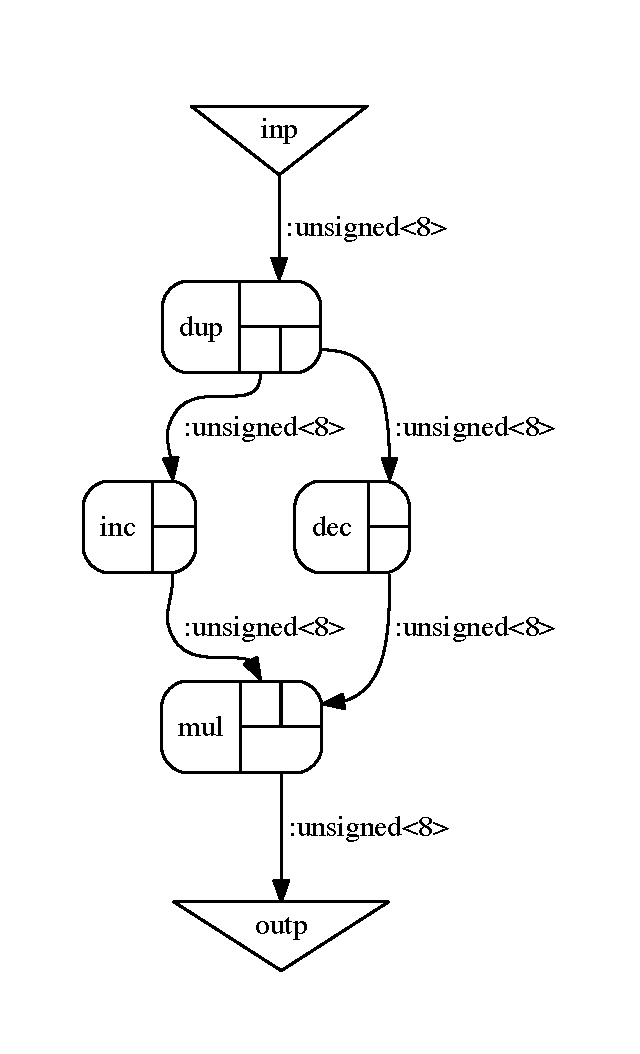
\includegraphics[width=0.3\textwidth]{./figs/simple-dot.pdf}
  \caption{The graphical representation of the program given in Listing.~\ref{lst:simple-full} computed
    by the \caph compiler front-end} 
  \label{fig:simple-dot}
\end{figure}

\section{Simulating the program}
\label{sec:simulation}

% Before generating the VHDL code, it is generally useful to simulate to program in order to check
% that it actually computes the expected results.

There are actually two ways of simulating programs : either directly from the source code, using the
reference interpreter of the language\footnote{As demonstrated in Part 2, with the IDE}, or by using
the SystemC backend.

In both cases, input(s) and output(s) will be read (resp. written) to text files\footnote{Of
  course, for the final application, running the on target hardware platform, there will have to be
  a builtin mechanism for producing the stream(s) of input tokens and consuming the stream(s) of
  output tokens. In practice, this mechanism will take the form of a couple 
  of dedicated VHDL processes reading and writing values from/to the I/O devices attached to the
  hardware platform (video cameras, digital display, host pc interface, \ldots).}.
Input text files can be simply written by hand or generated from other data representations (images,
in particulary) using ad-hoc conversion programs provided in the CAPH distribution (see Sec.~9.5 of
the reference manual). 

In our case, and in accordance to the
\verb|stream| declarations written in file \verb|simple.cph|, the input file will be named
\verb|sample.txt| and the output file \verb|result.txt|. The file \verb|sample.txt| simply contains
the sequence of input tokens (unsigned integers in this particular case, as shown in
Listing~\ref{lst:sample-input} :

\begin{lstlisting}[language=bash,frame=tb,caption={The input file \texttt{sample.txt} used for
    simulating the program of Listing~\ref{lst:simple-full}},label={lst:sample-input}]
1 2 3 4 5 6 7 8
\end{lstlisting}

\section{Simulation using the interpreter}
\label{sec:simul-using-interpr}

Simulation is launched by invoking the compiler with the \verb|-sim| option :

\begin{lstlisting}[style=BashInputStyle]
# caphc -sim simple.cph
\end{lstlisting}

Executing this command yields the following output 

\begin{lstlisting}[style=BashOutputStyle]
----------------------------------------------------------
This is the Caph compiler, version 2.8.3
...
Wrote file ./result.txt
----------------------------------------------------------
\end{lstlisting}

The contents of the file \verb|result.txt| is given in Listing~\ref{lst:sample-output}.

\begin{lstlisting}[language=bash,frame=tb,caption={The output file \texttt{result.txt} generated
    when simulating the program of Listing~\ref{lst:simple-full} with the input file of
    Listing~\ref{lst:sample-input}},label={lst:sample-output}]
0 3 8 15 24 35 48 63
\end{lstlisting}

\section{Simulation using the SystemC backend}
\label{sec:simul-using-syst}

This actually requires three steps : first generating the SystemC code representing the
application, second compiling this code to produce an executable and finally running this
executable.

The whole process is greatly simplified by using the \verb|caphmake| utility program included in
the distribution\footnote{Since version 2.8.1.}. This program automatically generates Makefile
descriptions from \emph{project} descriptions, describing the application-specific parameters. A
detailed presentation of \texttt{caphmake} can be found in Sec.~9.10 of the Reference Manual. We
will here only illustrate its basic usage.

\medskip Listing~\ref{lst:simple-proj-sysc} shows a very simple project file for compiling and
running the SystemC code derived from the \texttt{simple.cph} program. The \verb|SC_OPTS| macro
gives the options to pass the SystemC backend of the \texttt{caphc} compiler. 
Here the option \verb|-sc_stop_time| specifies the duration of the simulation in
\emph{ns}\footnote{The complete list of options is given in the language reference manual.}.

\begin{lstlisting}[style=MakeStyle,caption={File
    \texttt{simple.proj} for compiling and running SystemC code},label={lst:simple-proj-sysc}]
SC_OPTS = -sc_stop_time 200
\end{lstlisting}

\medskip
After writing \verb|simple.proj|, just invoke \texttt{caphmake} with the name of the main source
file :

\begin{lstlisting}[style=BashInputStyle]
# caphmake -main simple
\end{lstlisting}

This will write a file named \texttt{Makefile} in the current directory.

\medskip
Now use this top-level Makefile to generate the SystemC-specific makefile :

\begin{lstlisting}[style=BashInputStyle]
# make systemc.makefile
\end{lstlisting}

This will write a file named \texttt{Makefile.systemc} in the current directory.

\medskip
We now can generate the SystemC code by simply typing 

\begin{lstlisting}[style=BashInputStyle]
# make systemc.code
\end{lstlisting}

yielding the following output  

\begin{lstlisting}[style=BashOutputStyle,numbers=left,numberstyle=\tiny]
make -f Makefile.systemc code CAPH=/usr/local/caph
/usr/local/caph/bin/caphc -I /usr/local/caph/lib/caph -systemc -sc_stop_time 200 simple.cph
-------------------------------------------------------------------------------------------------
This is the Caph compiler, version 2.8.3
(C) 2011-2017 J. Serot (Jocelyn.Serot@univ-bpclermont.fr)
For more information, see : http://caph.univ-bpclermont.fr
-------------------------------------------------------------------------------------------------
Wrote file ./simple_expanded.dot
Wrote file ./simple_net.cpp
Wrote file ./dup_act.h
Wrote file ./dup_act.cpp
Wrote file ./mul_act.h
Wrote file ./mul_act.cpp
Wrote file ./dec_act.h
Wrote file ./dec_act.cpp
Wrote file ./inc_act.h
Wrote file ./inc_act.cpp
\end{lstlisting}

Line 2 shows the invocation of the \caph compiler with the SystemC backend.
Lines 8--17 show the different files generated by the \caph compiler. The file
\verb|simple_expanded.dot| is a variant of the file \verb|simple.dot| discussed in
Sec.~\ref{sec:drawing-network}\footnote{This variant, only required by the SystemC and VHDL backend,
  has explicit FIFO and flow-splitting nodes.}.  The file \texttt{simple\_net.cpp} contains the
top-level network description. The files \verb|dup_act.h| and \verb|dup_act.cpp| (resp. \verb|mul_act.h| and
  \verb|mul_act.cpp|, \verb|dec_act.h| and \verb|dec_act.cpp|, \verb|inc_act.h| and \verb|inc_act.cpp|)
  contain the interface and the implementation of the \verb|dup| (resp. \texttt{mul},
  \texttt{dec} and \texttt{inc}) actor.

\medskip
The generated code can be compiled by simply typing 

\begin{lstlisting}[style=BashInputStyle]
# make systemc.exe
\end{lstlisting}

yielding the following output, which shows the compilation of this code using the classical SystemC
flow (in our case, \verb|gcc|, with link to the \verb|systemc| library\footnote{Appropriate
  definitions are provided in the file \texttt{\$CAPH/lib/etc/Makefile.core} and can be adjusted according to your
  local SystemC installation.}).

\begin{lstlisting}[style=BashOutputStyle,numbers=left,numberstyle=\tiny]
make -f Makefile.systemc exe CAPH=/usr/local/caph
(cd .; g++ -std=c++11 -I. -I/usr/local/caph/lib/systemc -I/usr/local/systemc-2.3.1/include
  -Wno-deprecated -Wno-parentheses-equality -D_CPP11  -c `basename inc_act.cpp`)
(cd .; g++ -std=c++11 -I. -I/usr/local/caph/lib/systemc -I/usr/local/systemc-2.3.1/include
  -Wno-deprecated -Wno-parentheses-equality -D_CPP11  -c `basename dec_act.cpp`)
(cd .; g++ -std=c++11 -I. -I/usr/local/caph/lib/systemc -I/usr/local/systemc-2.3.1/include 
  -Wno-deprecated -Wno-parentheses-equality -D_CPP11  -c `basename mul_act.cpp`)
(cd .; g++ -std=c++11 -I. -I/usr/local/caph/lib/systemc -I/usr/local/systemc-2.3.1/include 
  -Wno-deprecated -Wno-parentheses-equality -D_CPP11  -c `basename dup_act.cpp`)
(cd .; g++ -std=c++11 -I. -I/usr/local/caph/lib/systemc -I/usr/local/systemc-2.3.1/include 
  -Wno-deprecated -Wno-parentheses-equality -D_CPP11  -c `basename simple_net.cpp`)
(cd .; g++ -L/usr/local/systemc-2.3.1/lib-macosx64 inc_act.o dec_act.o mul_act.o dup_act.o simple_net.o
   -o simple_sc -lsystemc  2>&1 | c++filt)
\end{lstlisting}

\medskip
Finally, simulation is launched by running the compiled executable

\begin{lstlisting}[style=BashInputStyle]
# make systemc.run
\end{lstlisting}

yielding the following output 

\begin{lstlisting}[style=BashOutputStyle,numbers=left,numberstyle=\tiny]
make -f Makefile.systemc run CAPH=/usr/local/caph
./simple_sc

        SystemC 2.3.1-Accellera --- Aug  9 2015 15:42:56
        Copyright (c) 1996-2014 by all Contributors,
        ALL RIGHTS RESERVED
Simulation stopped at t=200 ns
Wrote file result.txt
\end{lstlisting}

The generated file \verb|result.txt| contains the results of the simulation (which is exactly the
same as the one obtained when running the source level simulator).

\medskip
The three different steps (code generation, compilation, execution) can be run with a simple command
by simply typing \verb|make systemc.run| directly after invoking \verb|caphmake|.

\section{Generating and  simulating VHDL code}
\label{sec:generating-vhdl}

The \caph compiler can produce a complete RT-level VHDL representation of the application which can
be simulated and, latter synthetised using vendor specific tools (such as \textsc{altera} Quartus or
\textsc{xilinx} ISE). This section focuses on simulation (synthesis will be covered in
Sec.~\ref{sec:synth-vhdl-code}). 

\medskip
Classicaly, simulation of VHDL code is performed using dedicated simulators included in the vendor
toolsets (for example, the ALTERA Quartus toolset includes the \texttt{modelsim} simulator). We
describe here another approach, using a freely available VDHL compiler and simulator called
GHDL~\cite{GHDL}. GHDL can be invoked directly from the command line and hence can be easily
integrated in a makefile-based design-flow.

\medskip As for the SystemC backend, the \textbf{first step} is to define, in the project
description file (\verb|.proj|), all the application-specific options. In our case, the only thing
to do is add a line dedicated to the VHDL backend in the file described in
Listing~\ref{lst:simple-proj-sysc}, as shown in Listing~\ref{lst:simple-proj-vhdl}. 

\begin{lstlisting}[style=MakeStyle,caption={File
    \texttt{simple.proj} for compiling and running SystemC and VHDL code},label={lst:simple-proj-vhdl}]
SC_OPTS = -sc_stop_time 200
GHDL_RUN_OPTS = --stop-time=200ns
\end{lstlisting}

The added line (line 2) specifies to options to be passed to the GHDL simulator. 

\medskip
After that, the process is very similar to that described in the previous section for the SystemC
backend :

\begin{itemize}
\item invoke \verb|make vhdl.makefile| to build the VHDL-specific \textrm{Makefile},
\item invoke \verb|make vhdl.code| to generate the VHDL code,
\item invoke \verb|make vhdl.exe| to build the executable,
\item invoke \verb|make vhdlrunexe| to run the simulation.
\end{itemize}

As before, the three last steps can be obtained by simply typing 

\begin{lstlisting}[style=BashInputStyle]
# make vhdl.run
\end{lstlisting}

yielding, in our case, the following output 

\begin{lstlisting}[style=BashOutputStyle,numbers=left,numberstyle=\tiny]
make -f Makefile.vhdl run CAPH=/usr/local/caph
/usr/local/caph/bin/caphc -I /usr/local/caph/lib/caph -vhdl  simple.cph
-------------------------------------------------------------------------------------------------
This is the Caph compiler, version 2.8.3
(C) 2011-2017 J. Serot (Jocelyn.Serot@univ-bpclermont.fr)
For more information, see : http://caph.univ-bpclermont.fr
-------------------------------------------------------------------------------------------------
Wrote file ./simple_expanded.dot
Reverting to default size for fifo F12
Reverting to default size for fifo F11
Reverting to default size for fifo F10
Reverting to default size for fifo F9
Reverting to default size for fifo F8
Reverting to default size for fifo F7
Wrote file ./simple_net.vhd
Wrote file ./dup_act.vhd
Wrote file ./mul_act.vhd
Wrote file ./dec_act.vhd
Wrote file ./inc_act.vhd
Wrote file ./simple_tb.vhd
warning: VHDL annotation file fifo_caps.dat does not exist.
(cd .; ghdl -a -P/usr/local/caph/lib/vhdl `basename simple_tb.vhd`)
(cd .; ghdl -a -P/usr/local/caph/lib/vhdl `basename inc_act.vhd`)
(cd .; ghdl -a -P/usr/local/caph/lib/vhdl `basename dec_act.vhd`)
(cd .; ghdl -a -P/usr/local/caph/lib/vhdl `basename mul_act.vhd`)
(cd .; ghdl -a -P/usr/local/caph/lib/vhdl `basename dup_act.vhd`)
(cd .; ghdl -a -P/usr/local/caph/lib/vhdl `basename simple_net.vhd`)
(cd .; ghdl -e -P/usr/local/caph/lib/vhdl simple_tb)
/usr/local/caph/bin/txt2bin uint 8 sample.txt > sample.bin
ghdl -r -P/usr/local/caph/lib/vhdl simple_tb --stop-time=200ns --vcd=simple_tb.vcd 
./simple_tb:info: simulation stopped by --stop-time
\end{lstlisting}

Line 2 shows the invocation of the \caph compiler with the VHDL backend. The produced files are
listed on lines 15--20. The file \texttt{simple\_net.vhd} contains the top-level network
description, The files \verb|{dup_act.vhd|, \verb|mul_act.vhd|, \verb|dec_act.vhd| and
  \verb|inc_act.vhd| contain the RTL description of the actors involved in this network. The file
  \verb|simple_tb.vhd| contains a testbench for performing the simulation at the RTL
  level. Simulation itself is performed as shown in line 30.

  Line 29 shows the invocation of the \verb|txt2bin| utility program to generate the file
  \verb|sample.bin| to be used as input for simulation. The reason for this is that the input data
  files read by the VHDL code use a special, text-encoded binary format. The \verb|txt2bin| program
  is used to convert the input simulation file \verb|sample.txt| to this format\footnote{The extra
    arguments to the program, \texttt{uint 8} in this case, are infered from the type of the
    corresponding input stream. A complete description of the binary format and the associated
    converter programs is provided in the reference manual.}.

Simulation results are produced in file \verb|result.bin|. This file is encoded using the same
binary format and can be decoded using the \verb|bin2txt| utility program. For this, it suffices to
invoke 

\begin{lstlisting}[style=BashInputStyle]
# make vhdl.show
\end{lstlisting}

This yields the following result, which shows the expected values in file \texttt{result.txt}

\begin{lstlisting}[style=BashOutputStyle,numbers=left,numberstyle=\tiny]
make -f Makefile.vhdl show CAPH=/usr/local/caph
/usr/local/caph/bin/bin2txt uint 8 result.bin > result.txt
result.txt: 0 3 8 15 24 35 48 63 
\end{lstlisting}

\medskip
The ``functional'' style of simulation illustrated above is in general sufficient for assessing the
code. It is however possible to get a more ``time oriented'' view by using the \verb|--vcd| option
of the GHDL compiler. This option must be added to the macro \verb|GHDL_RUN_OPTS| in the project
file, as shown in Listing~\ref{lst:simple-proj-vhdl2}.

\begin{lstlisting}[style=MakeStyle,caption={File
    \texttt{simple.proj} for compiling and running SystemC and VHDL code (2nd
    version)},label={lst:simple-proj-vhdl2}]
SC_OPTS = -sc_stop_time 200
GHDL_RUN_OPTS = --stop-time=200ns --vcd=simple_tb.vcd
\end{lstlisting}

This instructs the GHDL simulator to dump a detailed \emph{log} of the simulation in VCD
format~\cite{VCD}. This log file can examined using various waveform visualisation
programs. Fig.~\ref{fig:simple-waves}, for example, shows an excerpt of the log file as visualized
by the \verb|gtkwave| application~\cite{gtkwave}. Visualisation has been here limited to signals
connected to the instance of the \verb|inc| actor. One immediately spots the \verb|clock| and
\verb|reset| signals\footnote{The clock period is set by default to 10 ns. There's an option of the
  compiler to change it (see~\cite{caph-lrm}.}.  The signal \verb|i_empty| goes to 0 when a data is
available on the FIFO connected to input \verb|i| of the actor. Reading from the FIFO is then
triggered by setting signal \verb|i_rd| to 1. Symetrically, the signal \verb|o_full| is 0 when place
is available on the FIFO connected to output \verb|o| of the actor. Writing to this FIFO is then
triggered by setting signal \verb|i_wr| to 1.

\begin{figure}[htbp]
  \centering
 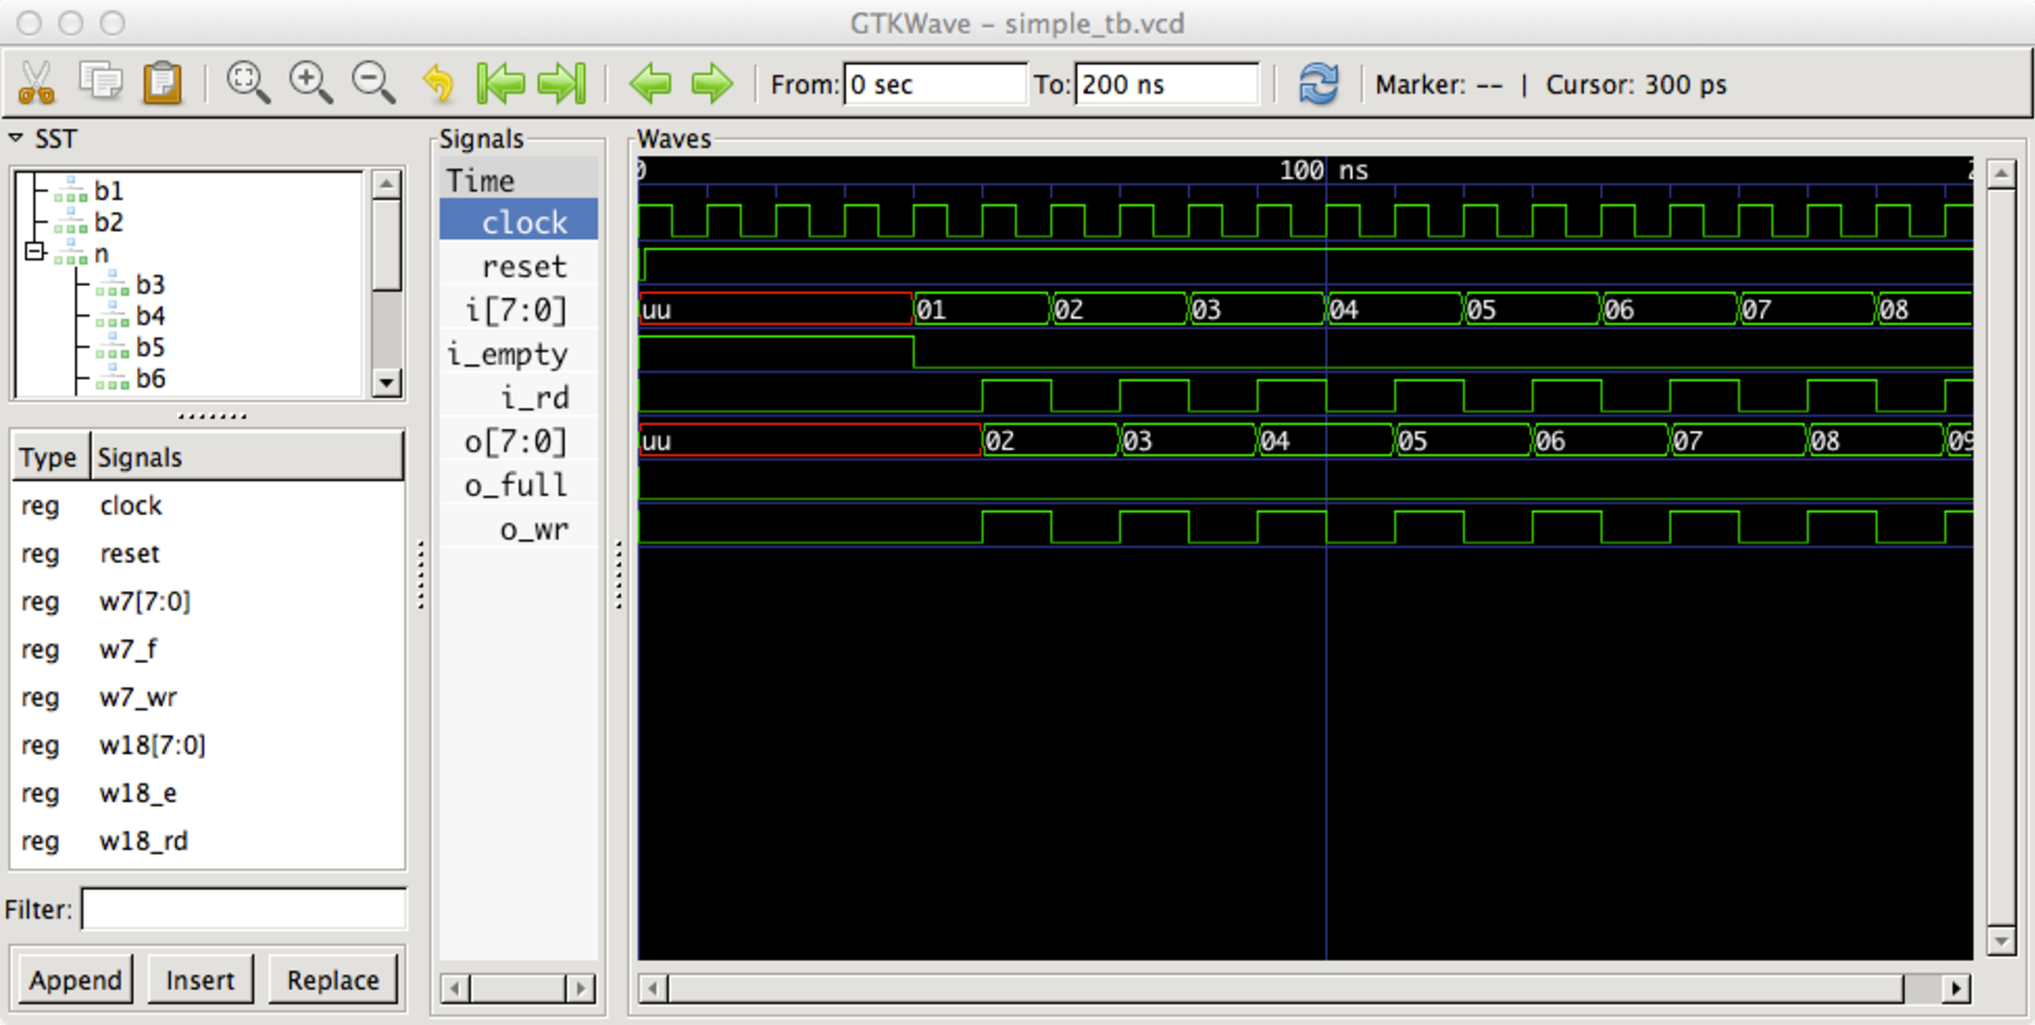
\includegraphics[width=\textwidth]{./figs/simple-waves.pdf}
  \caption{Some VHDL simulation results as viewed by \texttt{gtkwave}} 
  \label{fig:simple-waves}
\end{figure}

\section{Synthetizing the VHDL code}
\label{sec:synth-vhdl-code}

By synthesis we mean the tranformation of the RT-level code generated by the \caph compiler into a
FPGA configuration. Contrary to simulation, this operation depends on the physical target device and
requires the toolset from the corresponding vendor.  We do not address the issue of physical I/O
interfacing -- \emph{i.e.} we only describe the synthesis of the ``core'' functionality described by
the CAPH network (integration of CAPH-generated code into a full-fledged hardware platform is can be
carried out with the \textsc{GpStudio} IDE by example~\cite{GpStudio}).

In this section, we will illustrate the process
with the Quartus II suite of tools from \textsc{altera}, using the \verb|simple| application\footnote{This is
  only for pedagogical reasons since this application is obviously not a very useful one.
  Chap.\ref{cha:cl-images} and \ref{cha:cl-ip} will show how to implement more ``realistic'' applications,
  performing image processing.}.

\medskip Figs.\ref{fig:simple-quartus-1} to \ref{fig:simple-quartus-4} illustrates the creation of
the relevant project under the Quartus II (version 13.1) environment\footnote{We make the assumption
  here that the reader has a minimum familiarity with this environment. Several good tutorials can
  be found online, in particular on the ALTERA website.}.

Fig.~\ref{fig:simple-quartus-1} shows the
main Quartus window just after launching. In this window, select \textsf{File} in the top menu bar and
then the \textsf{New Project Wizard} item.

A window named after this item pops up. Fill the requested text
fields as illustrated in Fig.~\ref{fig:simple-quartus-2}. In our case, we have copied all the VHDL
files generated by the \caph compiler in a separate directory named
\verb|Z:/vhdl/caph/simple|\footnote{The option \texttt{-vhdl\_target\_dir} of the compiler can be
  used for that purpose.}. The
name of the project and the name of the top-level design entity must be set to
\verb|simple_net|. Clicking on the \textsf{Next} butten then brings the window shown in
Fig.~\ref{fig:simple-quartus-3}.

In this window, using the \textsf{...} and \textsf{Add} buttons, you have to specify the list of all the
VHDL files included in the projet. In our case, two groups of files are added : the five files
generated by the \caph compiler : \verb|dup_act.vhd|, \verb|mul_act.vhd|, \verb|dec_act.vhd|,
  \verb|inc_act.vhd| and \verb|simple_tb.vhd|; and two predefined files taken from the \caph VHDL
  library : \verb|../lib/caph.vhd| and \verb|../lib/fifo_fb.vhd| (the former contains a set of types
  and functions related to the \caph language, the latter the implementation of a generic
  FIFO). When completed, click again on the \textsf{Next} button.

  This brings up the window shown in Fig.~\ref{fig:simple-quartus-4}, in which you select the target
  device. In our case, a simple Cyclone III is chosen. Clicking then on the \textsf{Finish} button
  brings back to main window.

  On the \textsf{Project Navigator} subwindow (top left), select \textsf{Hierarchy} to show the design
  hierarchy. Selecting an entity will then print the corresponding source file on the right
  subwindow, as illustrated in Fig.~\ref{fig:simple-quartus-5}.

Synthesis is launched by selecting the \textsf{Start Compilation} item in the \textsf{Processing} menu
(or simply by clicking the small right-oriented purple triangle in the toolbar). Depending on your
machine this may take from a few seconds to a few minutes. In our case, the result is shown in
Fig.~\ref{fig:simple-quartus-6}. Here, it can be noted that only a very small fraction of the
available hardware resources is used.  

Fig.~\ref{fig:simple-quartus-7} shows the RT-level view of the design after
synthesis\footnote{Before physical mapping. It is also possible to get a post-mapping view.}. This
is obtained by invoking the \textsf{Netlist viewer} item in the \textsf{Tools} menu.

\begin{figure}[htbp]
  \centering
 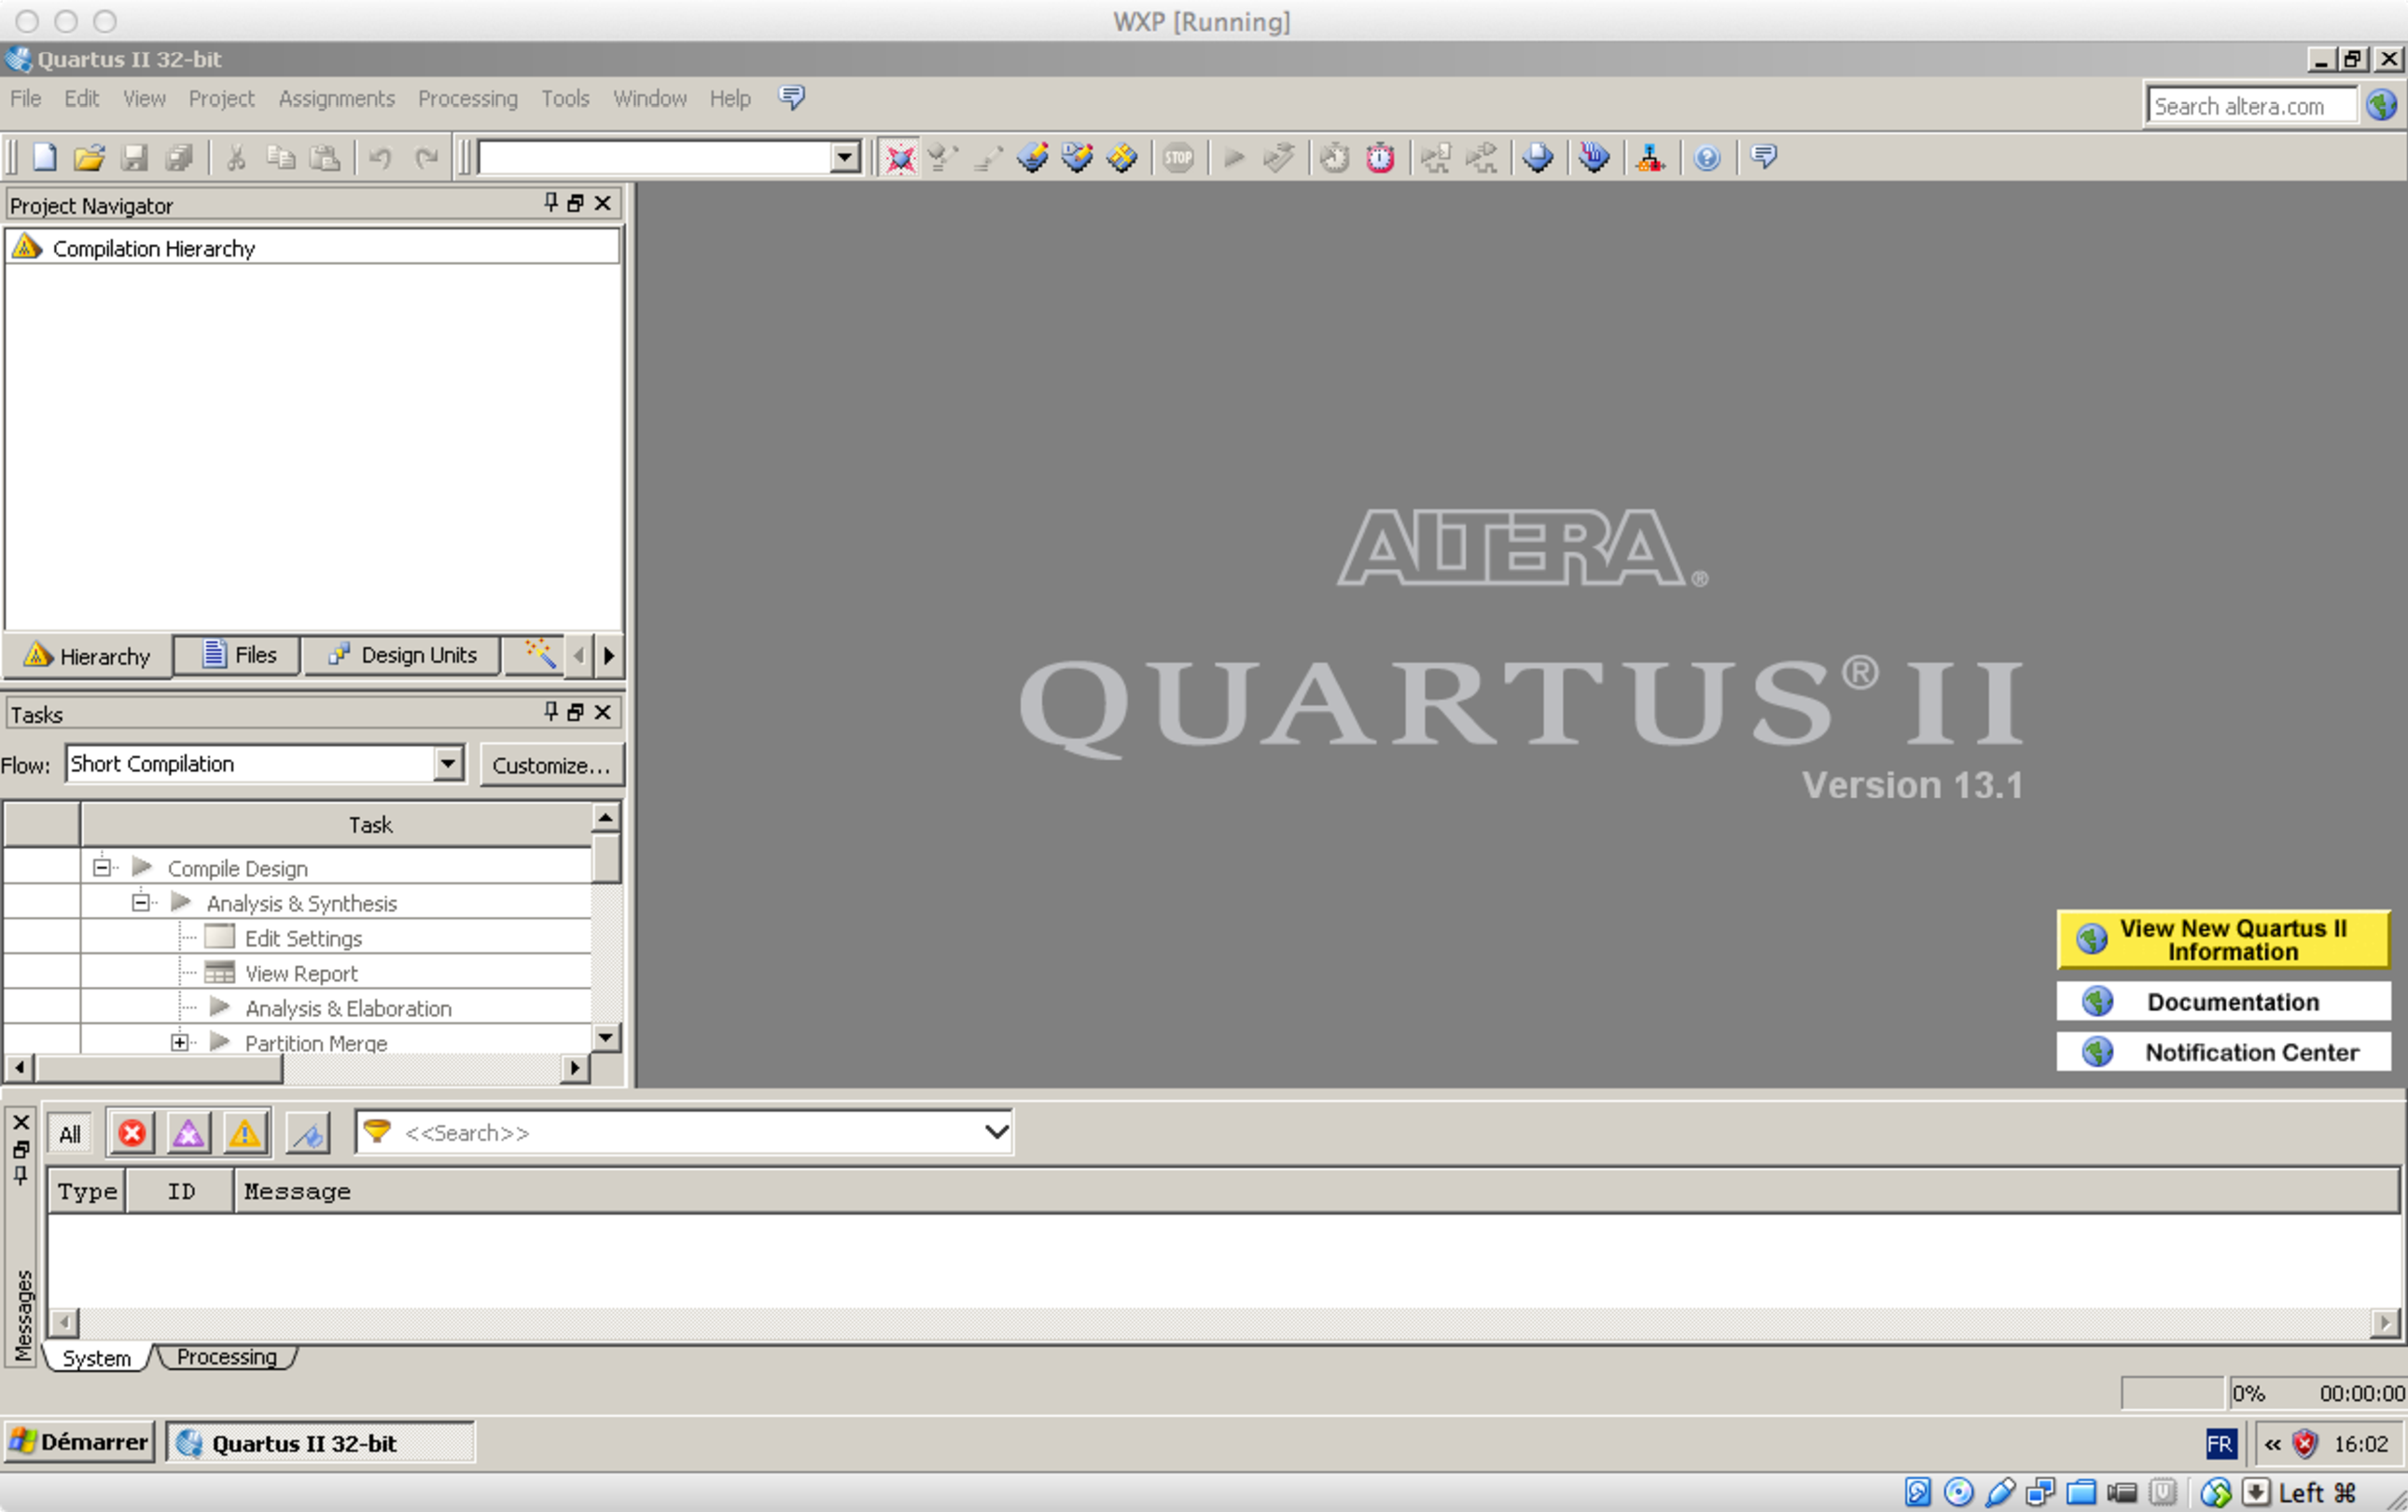
\includegraphics[angle=90,width=0.8\textwidth]{./figs/simple-quartus-1.pdf}
  \caption{The Quartus II environment, just after launching}
  \label{fig:simple-quartus-1}
\end{figure}

\begin{figure}[htbp]
  \centering
 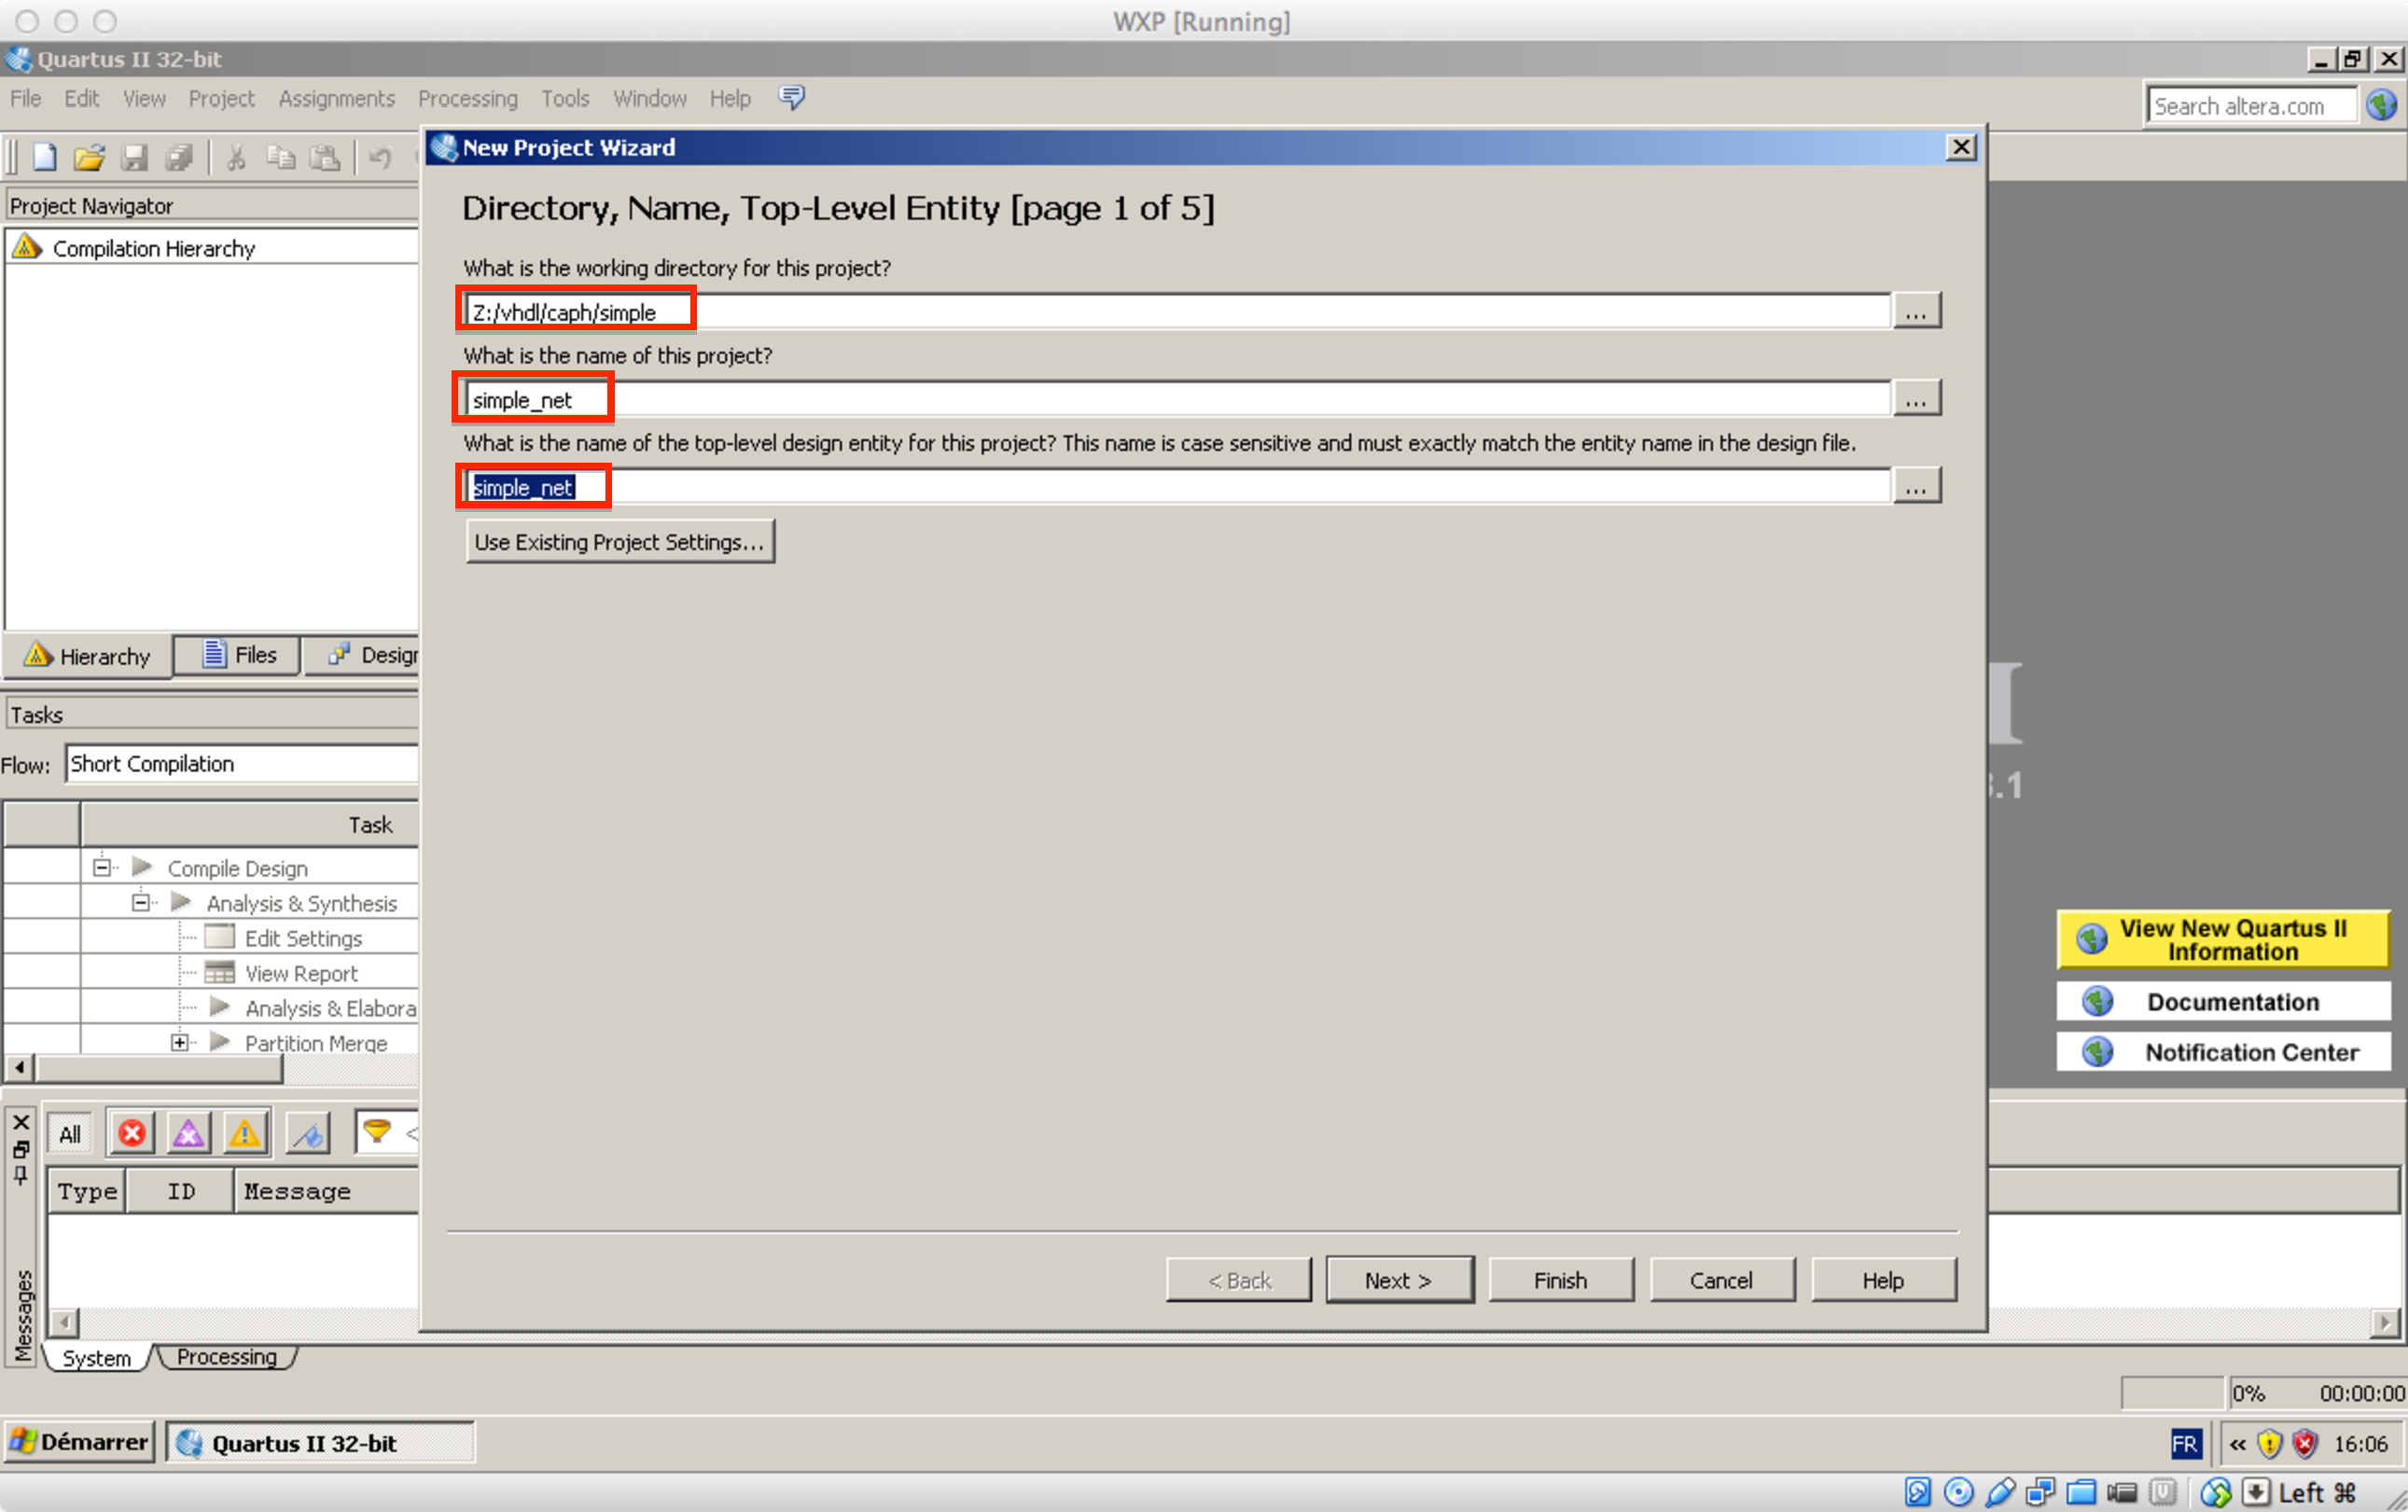
\includegraphics[angle=90,width=0.8\textwidth]{./figs/simple-quartus-2.pdf}
  \caption{Setting the projet - directory and top entity selection}
  \label{fig:simple-quartus-2}
\end{figure}

\begin{figure}[htbp]
  \centering
 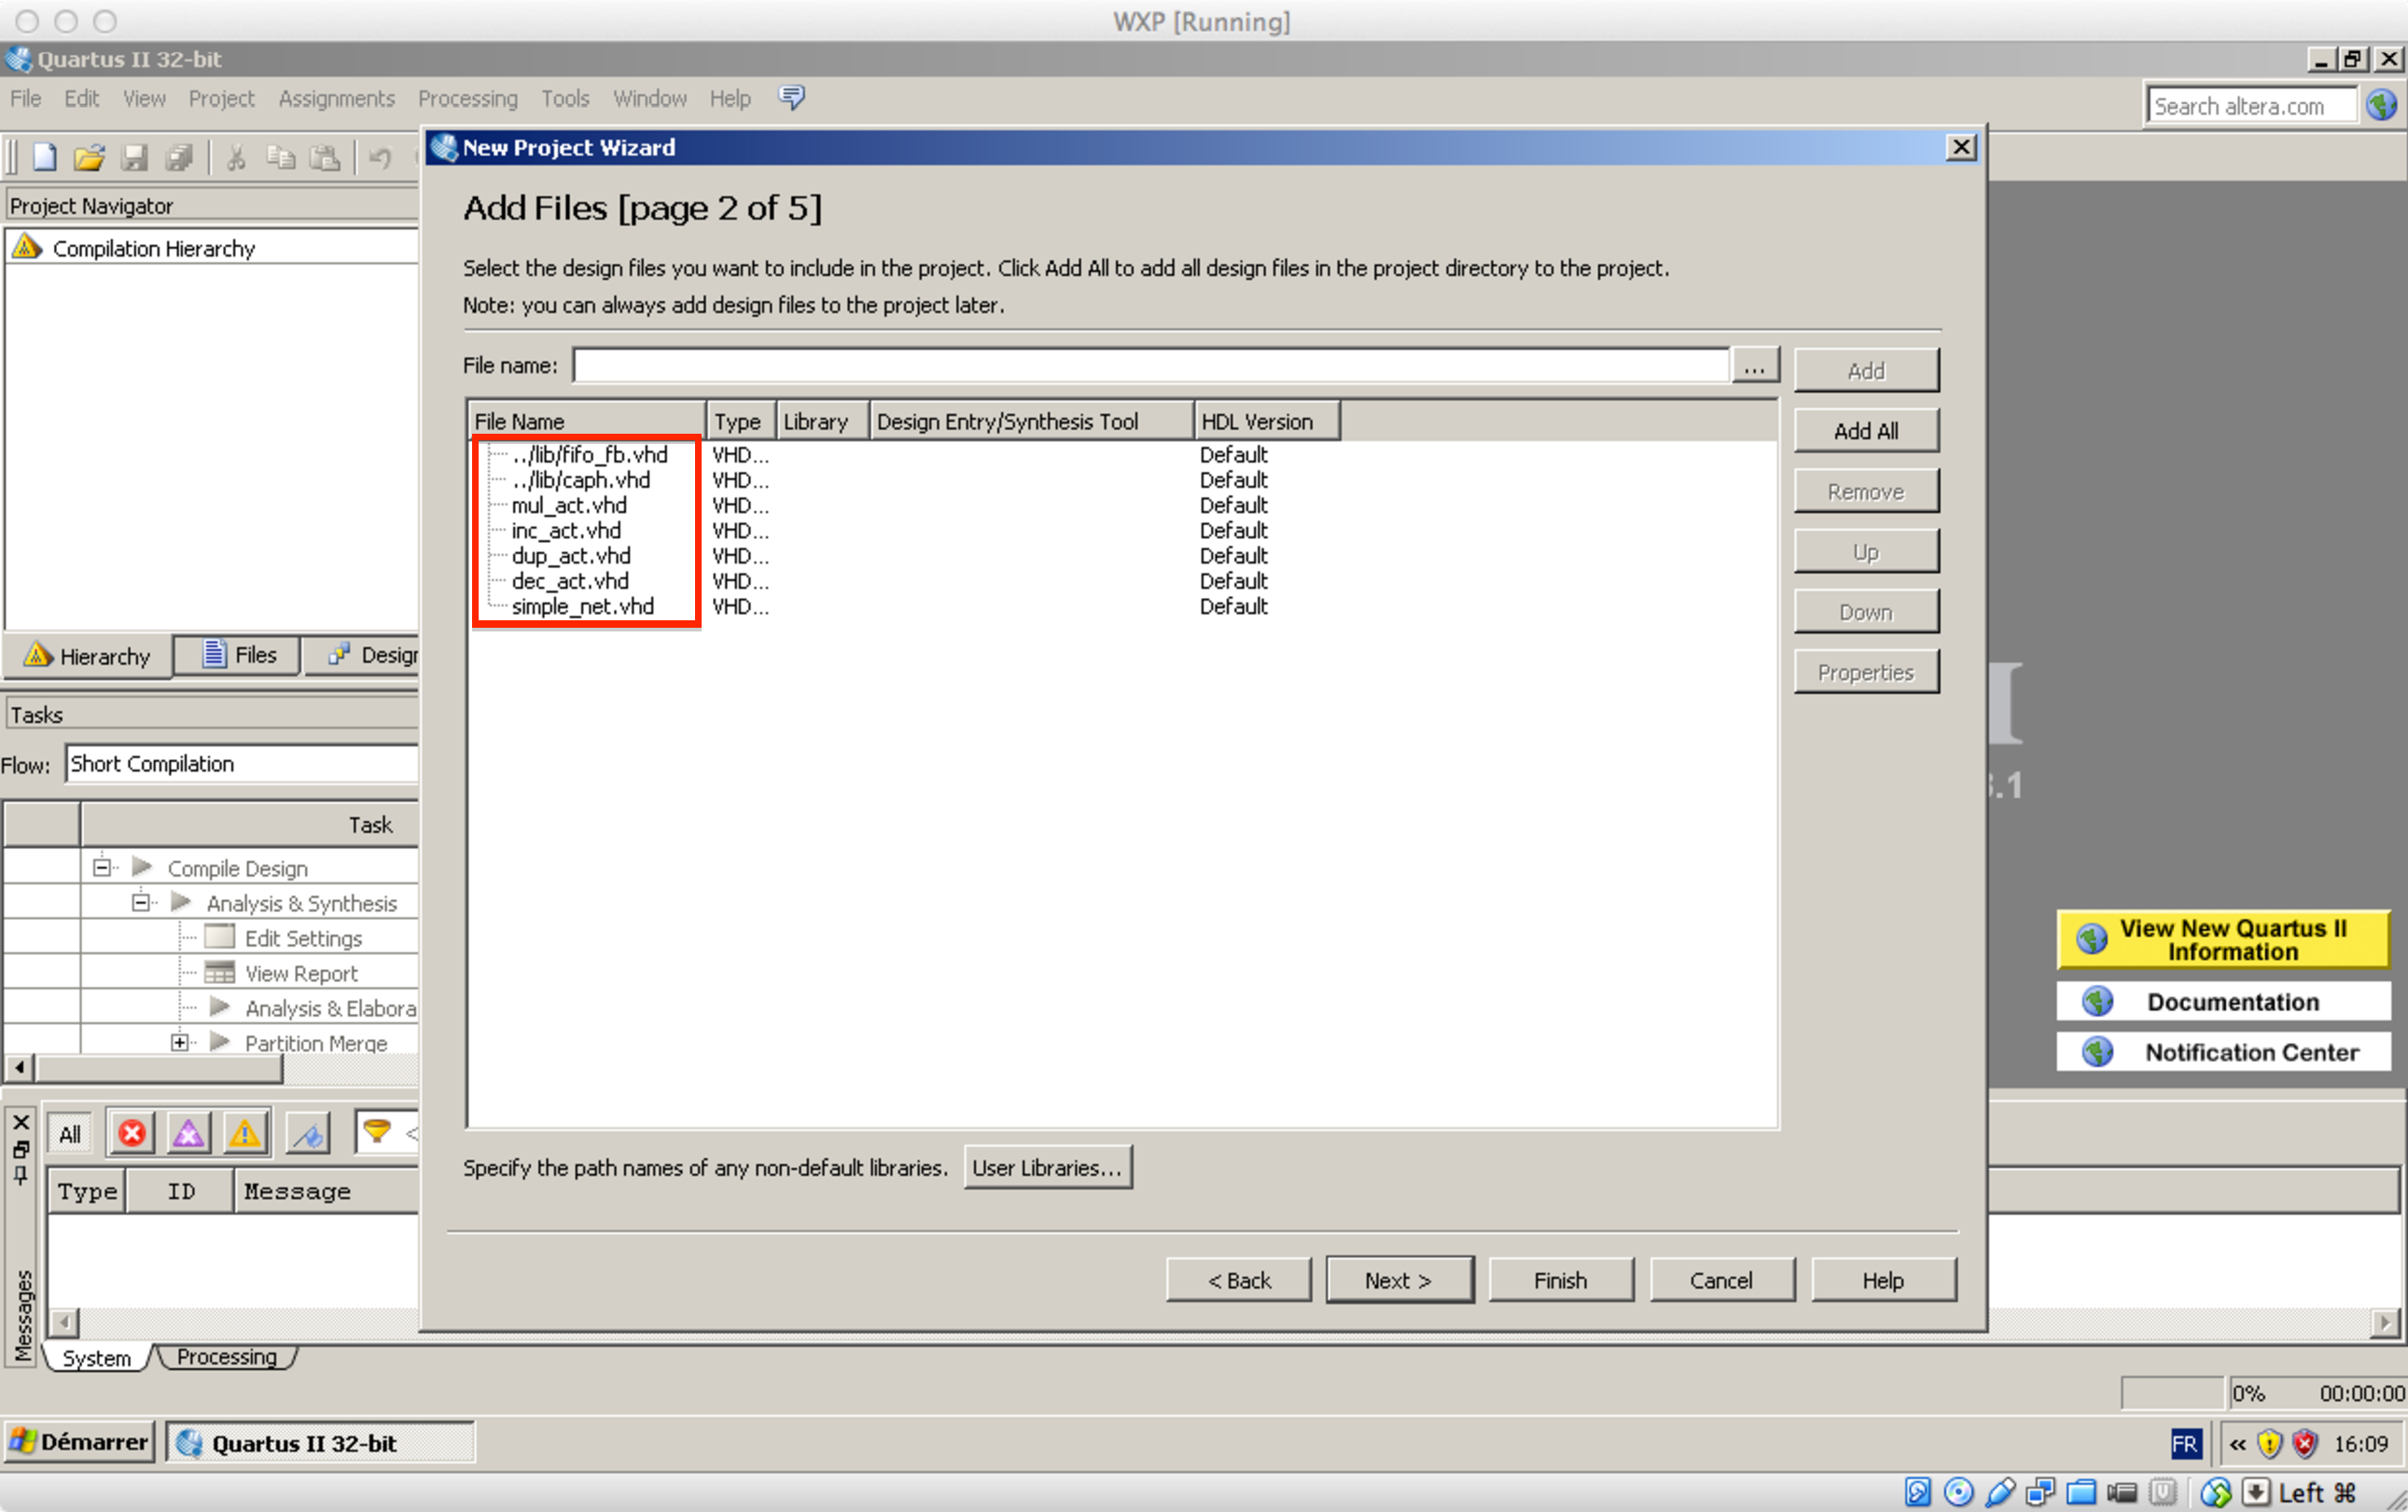
\includegraphics[angle=90,width=0.8\textwidth]{./figs/simple-quartus-3.pdf}
  \caption{Setting the source files of the project}
  \label{fig:simple-quartus-3}
\end{figure}

\begin{figure}[htbp]
  \centering
 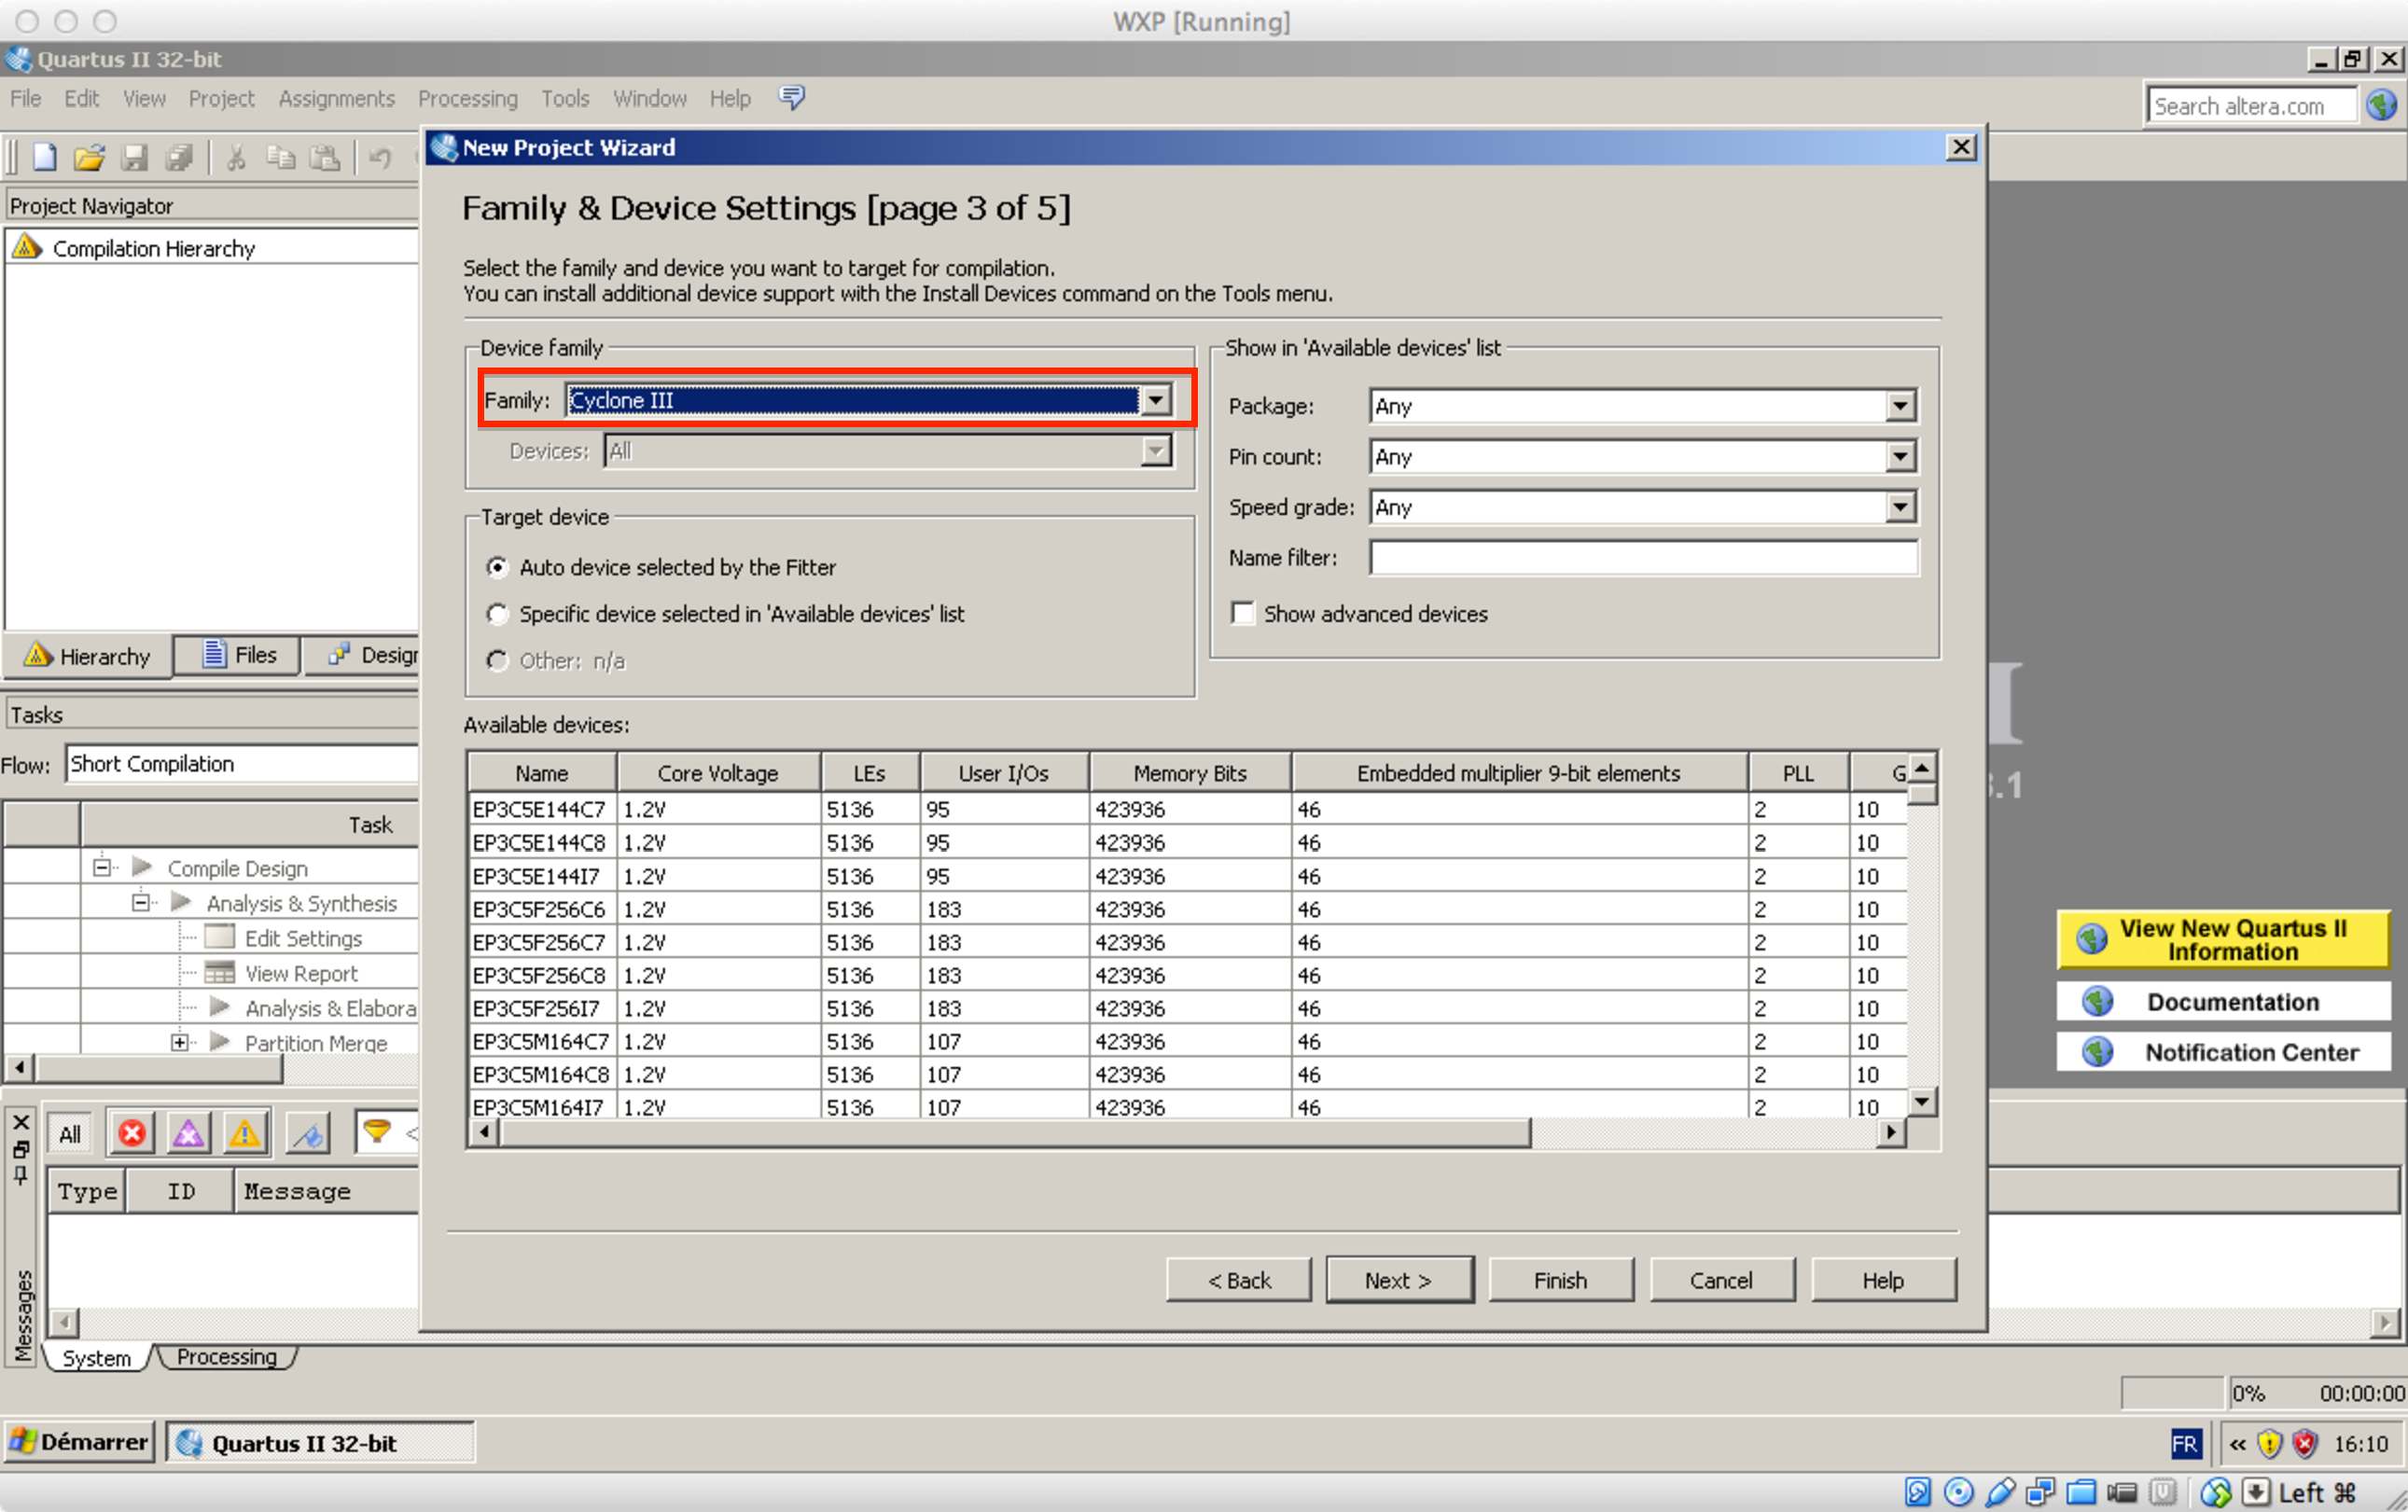
\includegraphics[angle=90,width=0.8\textwidth]{./figs/simple-quartus-4.pdf}
  \caption{Setting the target device}
  \label{fig:simple-quartus-4}
\end{figure}

\begin{figure}[htbp]
  \centering
 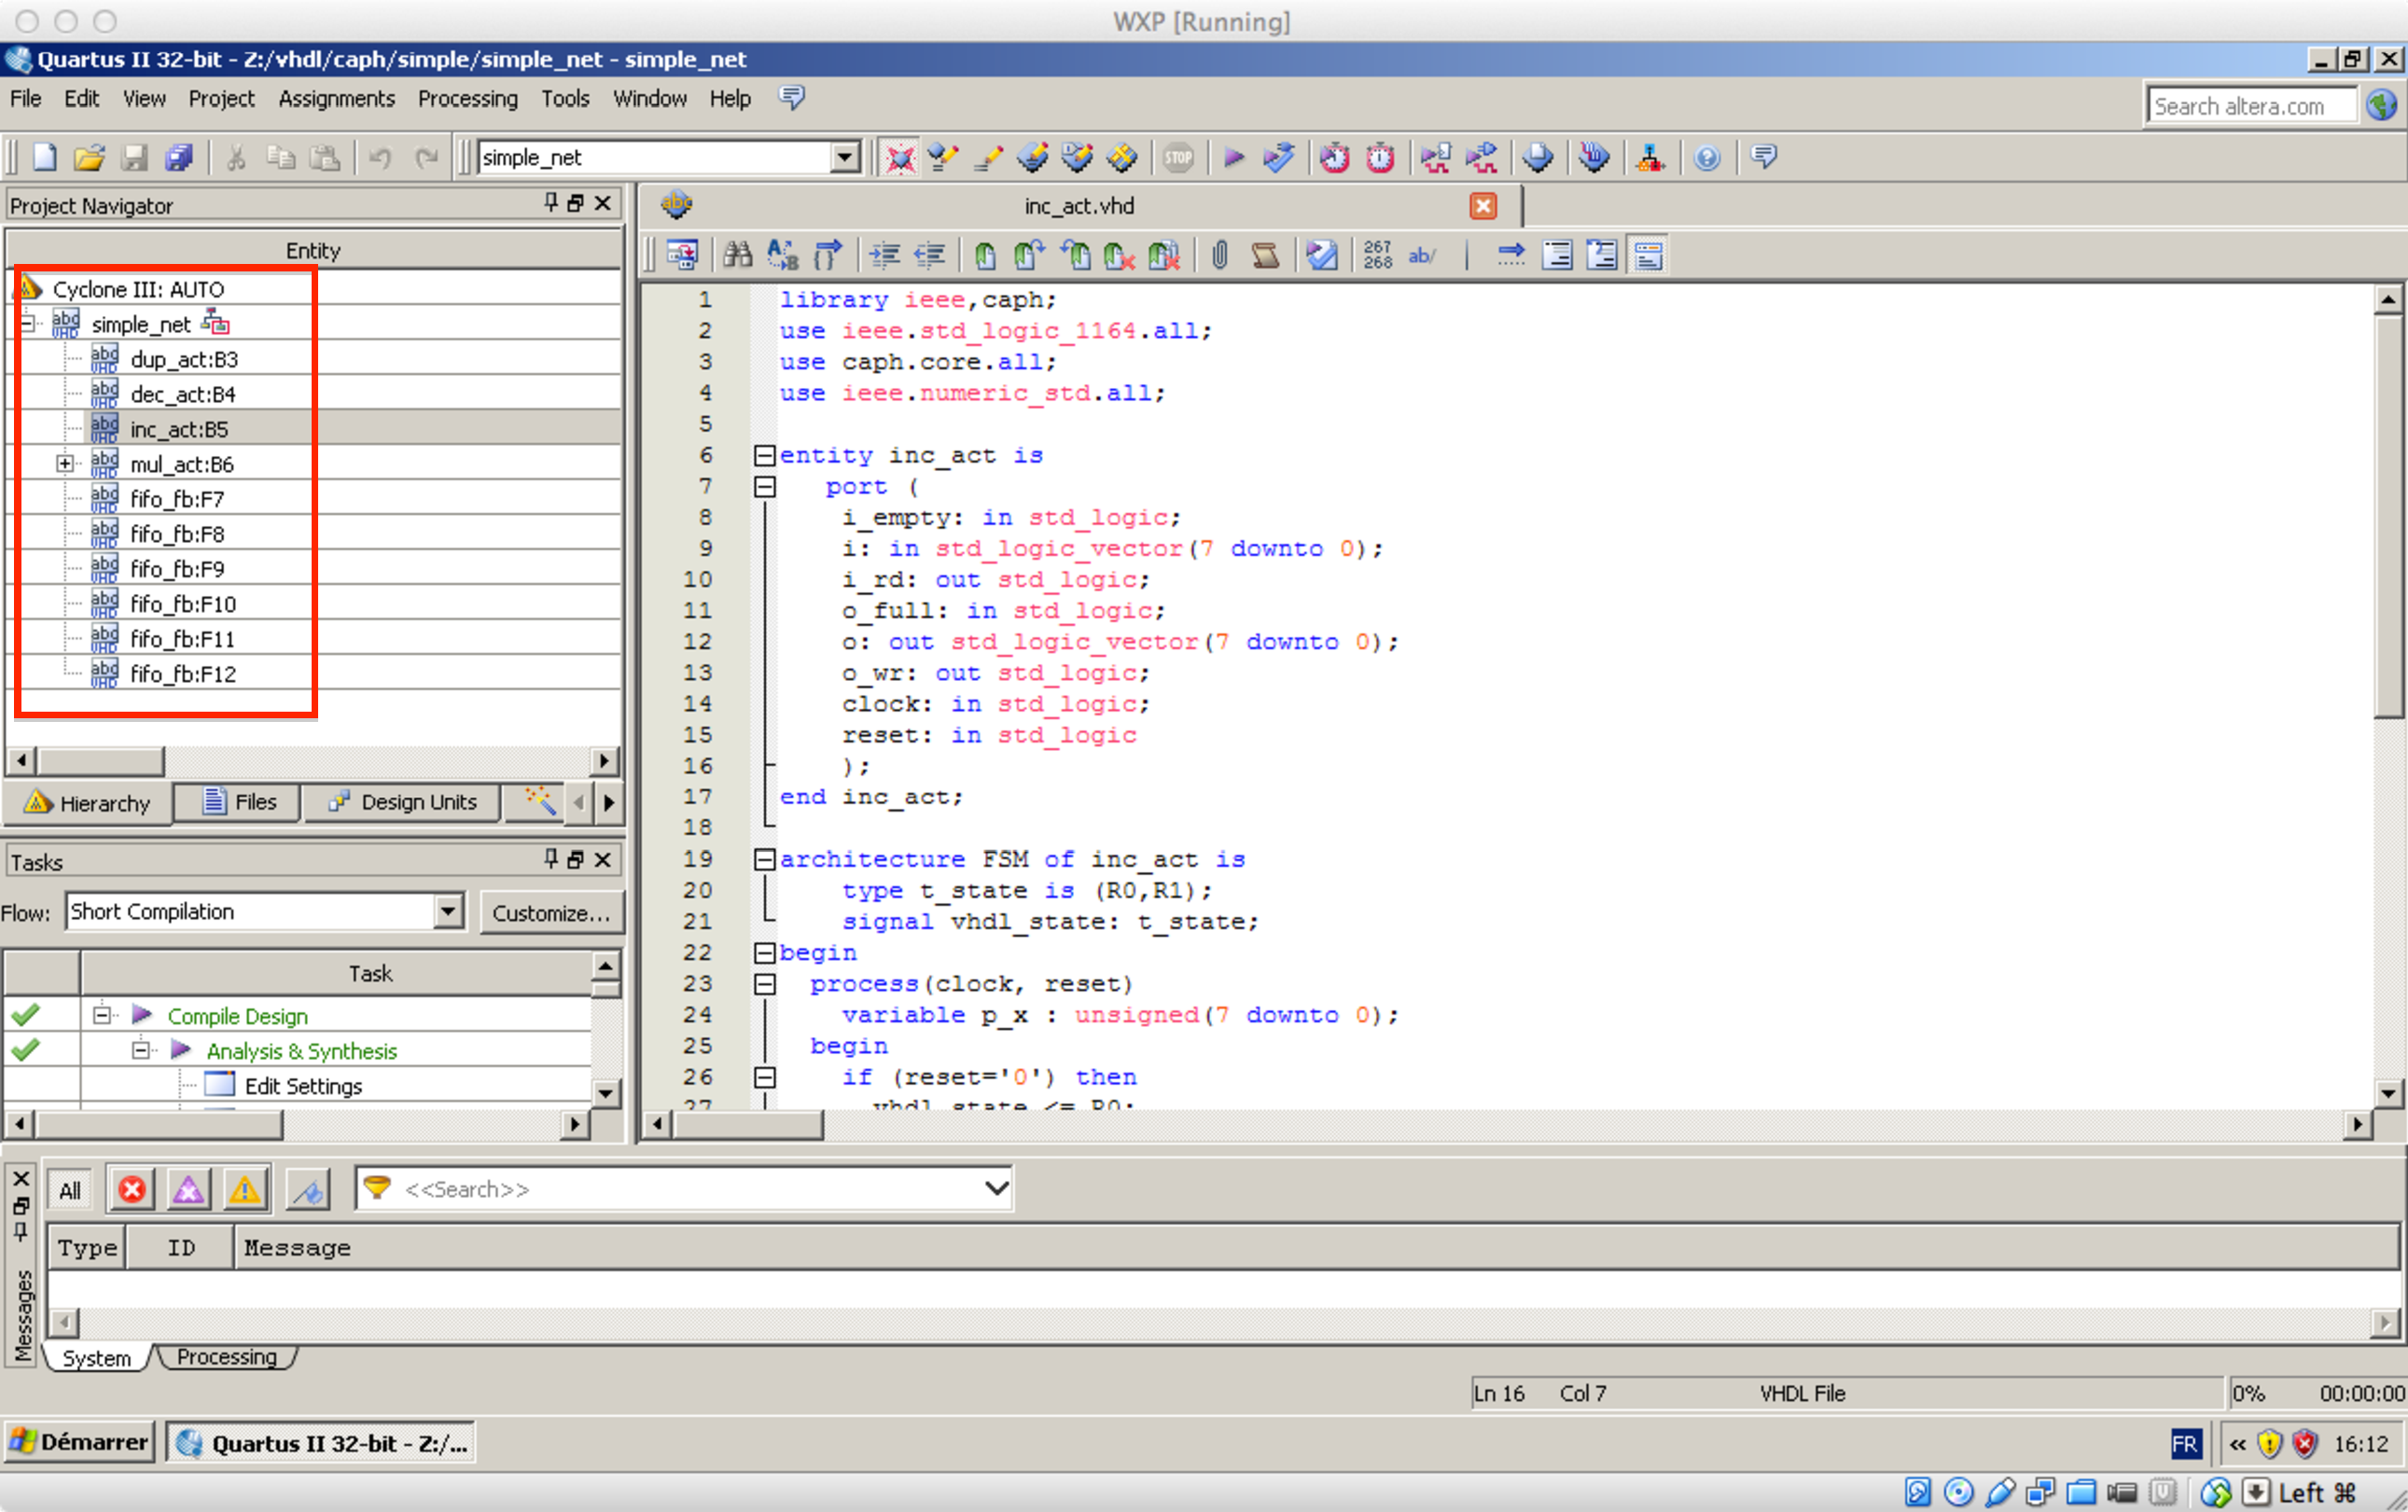
\includegraphics[angle=90,width=0.8\textwidth]{./figs/simple-quartus-5.pdf}
  \caption{Displaying design hierarchy and source files}
  \label{fig:simple-quartus-5}
\end{figure}

\begin{figure}[htbp]
  \centering
 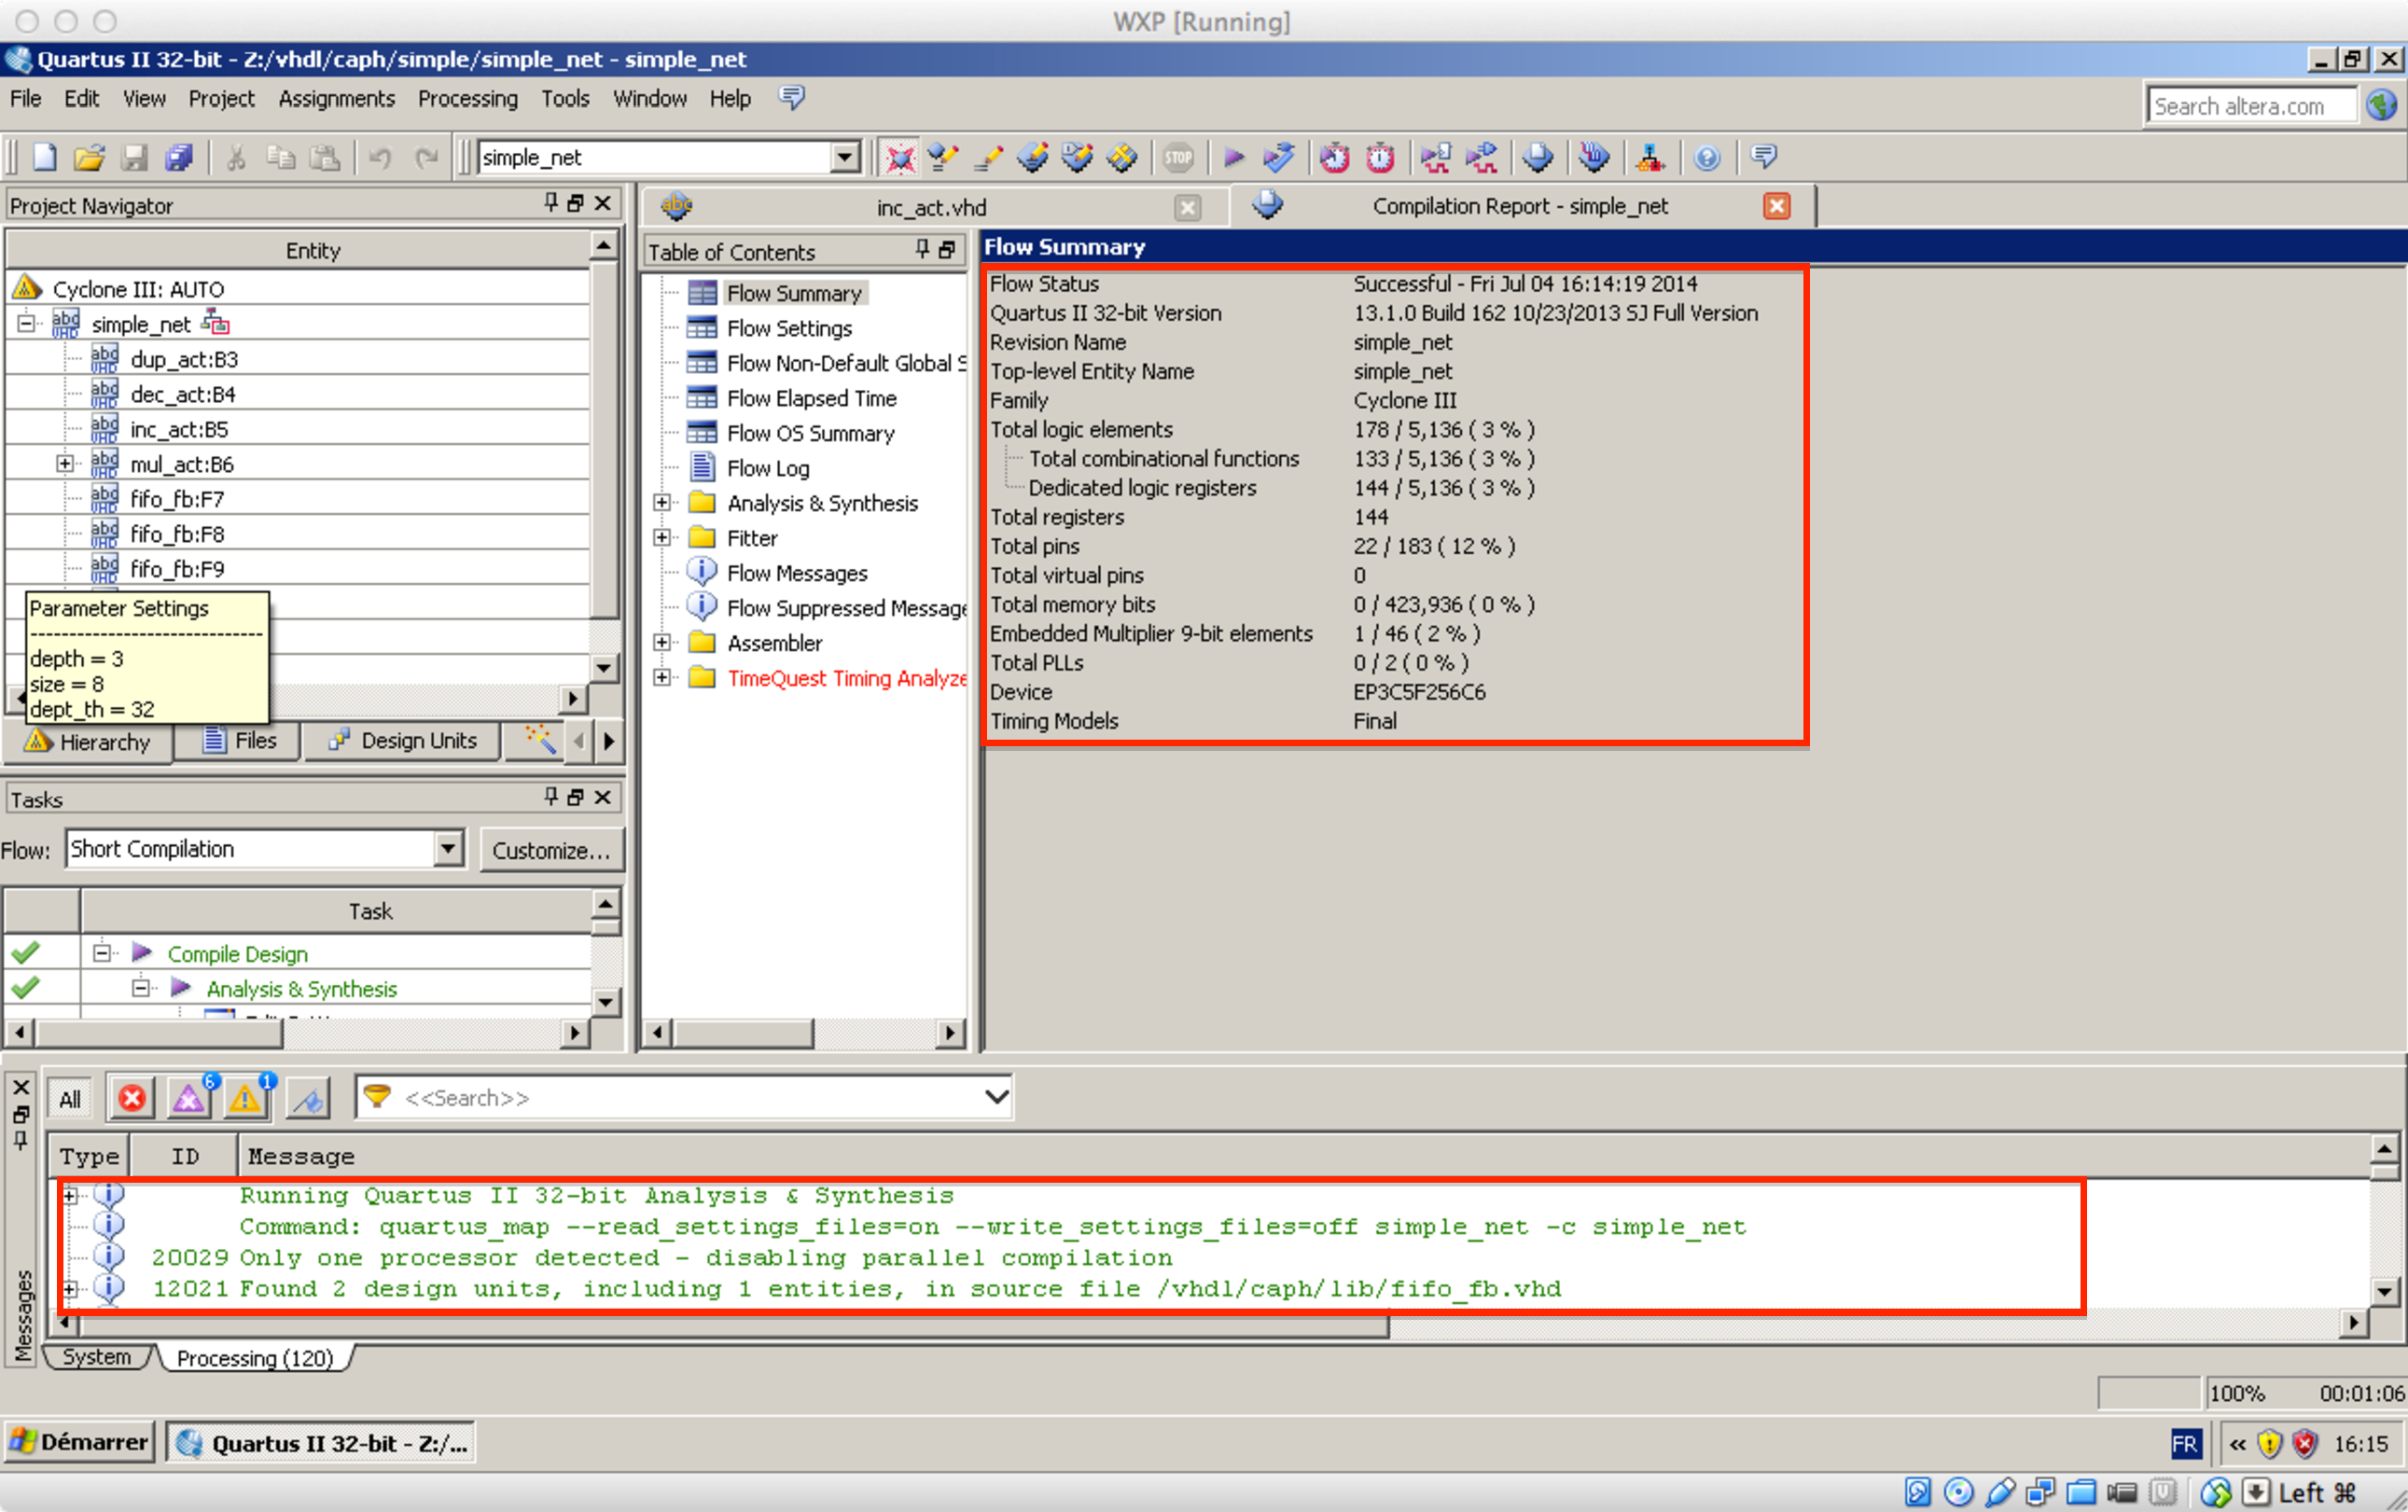
\includegraphics[angle=90,width=0.8\textwidth]{./figs/simple-quartus-6.pdf}
  \caption{Synthesis results}
  \label{fig:simple-quartus-6}
\end{figure}

\begin{figure}[htbp]
  \centering
 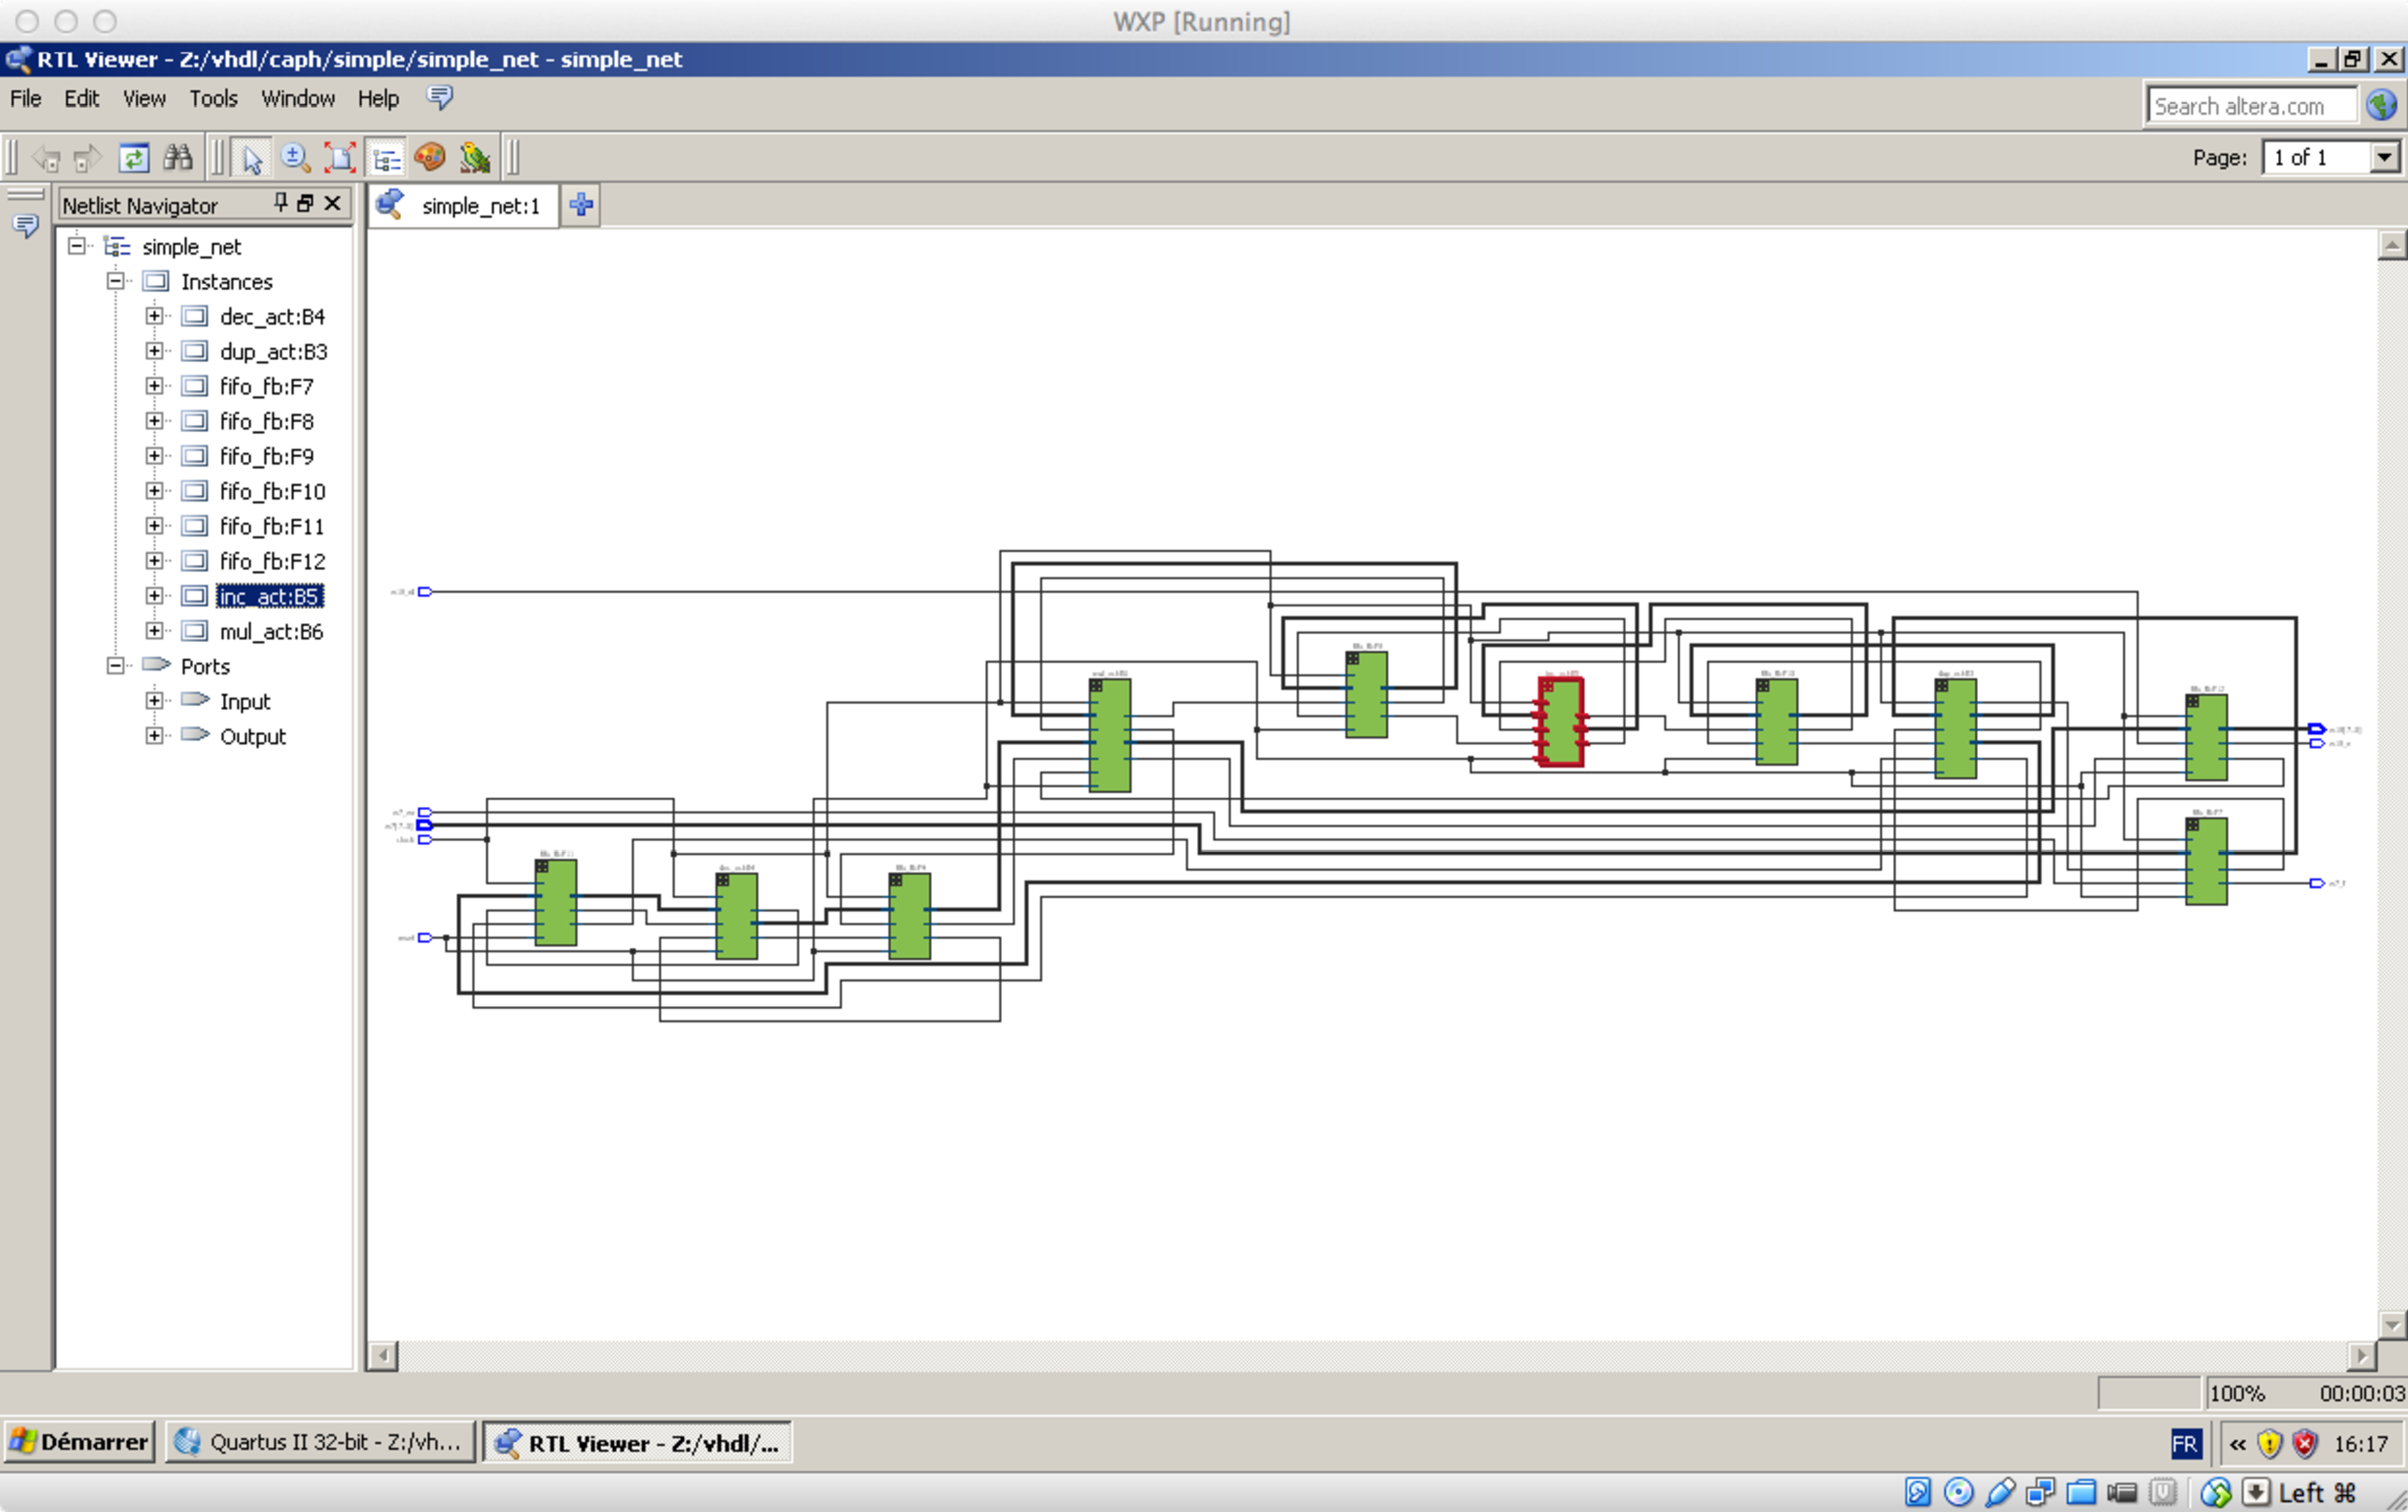
\includegraphics[angle=90,width=0.8\textwidth]{./figs/simple-quartus-7.pdf}
  \caption{Post-synthesis, RT-level view}
  \label{fig:simple-quartus-7}
\end{figure}

%%% Local Variables: 
%%% mode: latex
%%% TeX-master: "caph-primer"
%%% End: 
